\chapter{Results and Discussion}

\section{Introduction}
In this chapter, The results of the developed models are tabulated and discussed. Moreover, the evaluation of the proposed model for each problem is presented. Every model is tested using the metrics that suites its objective. In the following sections, virtual flow meter results are presented then the predictive maintenance. Finally, the optimal policy and optimization learning rate for steam injection project is presented. 

\section{Results of the virtual flow meter}

\section{Results of predictive maintenance of ESPs}
To reduce the false alarms in our model, the raw-sensor data have been pre-processed. Then, the “cleaned standardized” time-series data with their moving difference are entered into feature engineering transformation through the use of \ac{PCA}. Finally, A Machine learning models is used to classify the operating points conditions.

The upcoming results are reported in two different processes. Firstly, a validation results are reported using the 10 folds validation. Along with model training, model validation intends to locate an ideal model with the best execution. The model performance is optimized using training and validation data set. Therefore, \ac{ROC} curves are reported for the 10 folds of the dataset and their mean value. Then, the model generalization performance is tested using testing set. The test data set remains hidden during the model training and model performance evaluation stage. In this regard, precision recall curve is used.

Figure 8 shows the fraction of correct predictions for the positive class depicted on the y-axis versus the fraction of errors for the negative class depicted on the x-axis. For interpreting the \ac{ROC} curve, a single score can be given for a classifier model through the so-called “ROC area under curve” (AUC), which is attained -as the name implies- by integrating the area under the curve. The score has a value ranging between 0.0 and 1.0 which indicates a perfect classifier. Fig \ref{fig:ROC_PM} shows the ROC curves for our proposed model with 10-fold validation sets and its mean curve. The mean value for \ac{ROC} AUC is 0.95.

\begin{figure}
    \centering
    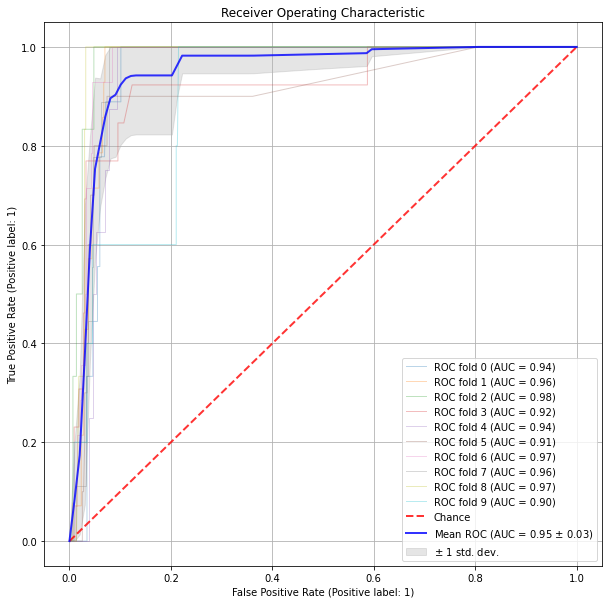
\includegraphics[width = \textwidth]{figures/predictive_maintenance/Fig 8-updated.png}
    \caption{ROC for the proposed model}
    \label{fig:ROC_PM}
\end{figure}

As mentioned earlier, the second process was testing the proposed model against a testing set using the precision-recall curve (PRC), which is a valuable diagnostic tool particularly when classes are very imbalanced. The PRC trade-off between a classifier’s precision, a measure of result relevancy, and recall, a measure of completeness for every possible cut-off, is depicted. Figure \ref{fig:PRC_PM} shows a precision recall curve PRC for the Pre-Workover and Workover class. 

  \begin{figure}
      \centering
      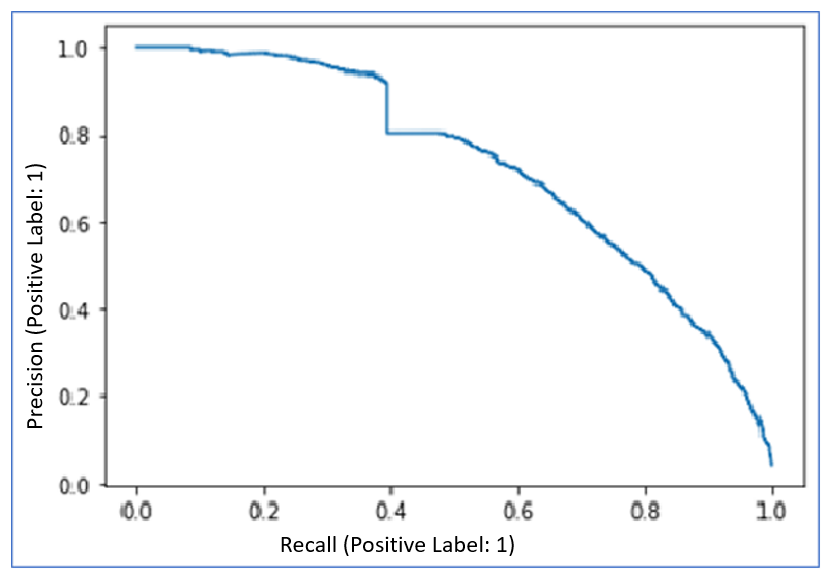
\includegraphics[width = \textwidth]{figures/predictive_maintenance/FIg 9.png}
      \caption{Precision Recall Curve}
      \label{fig:PRC_PM}
  \end{figure} 

It is clear that the dataset is unbalanced. For this reason, it is important to check the precision and recall for each class of the pumping conditions for better evaluation of the classifier. From Figure 9 and table \ref{tab:precision_pm}, The precision and the recall for pre-workover and workover condition is less than those in normal conditions. This is mainly due to a higher number of data points supporting the normal labelled status. This is an effect of using unbalanced dataset. One approach to addressing the imbalanced datasets is to oversample the minority class. The simplest approach involves duplicating examples in the minority class, although these examples don’t add any new information to the model. Instead, new examples can be synthesized from the existing examples. This is a type of data augmentation for the minority class and is referred to as the Synthetic Minority Oversampling Technique (SMOTE). This can be part of further work. However, such procedures are inherently dangerous because they may result in overfitting of the model.  

% Please add the following required packages to your document preamble:
% \usepackage{graphicx}
\begin{table}[]
\resizebox{\columnwidth}{!}{%
\begin{tabular}{l|l|l|l|l|}
\cline{2-5}
                                                   & precision & recall & f1-score & support \\ \hline
\multicolumn{1}{|l|}{Normal}                       & 0.99      & 1.00   & 1.00     & 101,726 \\ \hline
\multicolumn{1}{|l|}{seven days or less pre-event} & 0.80      & 0.60   & 0.71     & 604     \\ \hline
\end{tabular}%
}
\caption{Precision, Recall and F1 score}
\label{tab:precision_pm}
\end{table}

\section{Results of the steam injection optimization }
In this section we will examine the results of the learning process and the optimization of the steam injection rate through time. In particular we are interested in the learning curve exhibited by the agent, and the optimal steam injection rate policy obtained. 

Fig. \ref{fig:learning_curve_rl} shows the learning curve for our agent, where the line represents the cumulative net present value for each episode after 820 days. Large variations in the \ac{NPV} of initial episodes can be observed which is due to poor approximations of the actor network. Typically, the critic is a state-value function. After each actor selection, the critic evaluates the new state to determine whether things have improved or become worse than expected, the decisive parameter  called the temporal difference error (TD). As the number of episodes increases, the critic learns about whatever policy is currently being followed by the actor. This critique takes the form of a TD error. This scaler signal is the sole output of the critic and drives all learning in both actor and critic. 

\begin{figure}
    \centering
    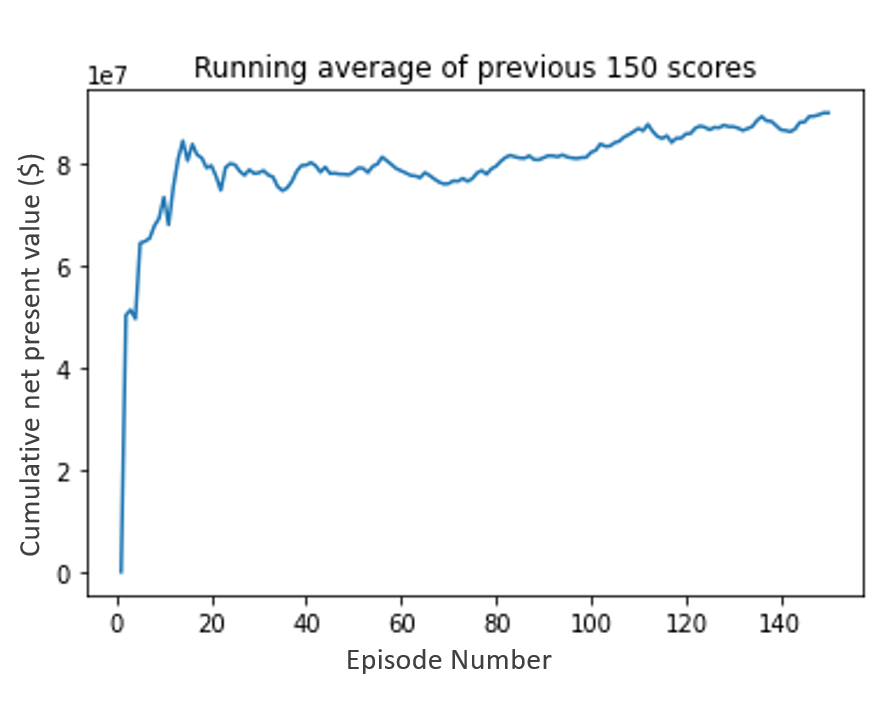
\includegraphics[width =\textwidth]{figures/prescriptive_analysis/learning_curve.png}
    \caption{Learning curve of RL}
    \label{fig:learning_curve_rl}
\end{figure}

Figure \ref{fig:FWIR} shows the optimal steam injection curves for the a2c agent and the base model versus time. Four specific regions can be distinguished in the optimal injection policy: from 0 to 380 days, the injection rate has slightly changed between 98 to 118 bbl/day. The second region is from 380 to 640 days where injection rate increased from 118 bbl/day to a maximum value 148 bbl/day. The third region (from 640 to 780) shows a steep decrease of the injection rate from 148 bbl/day to 98bbl/day. The fourth is from 780 to 820 showing a slight change between 98 bbl/day and 108 bbl/day. As per figure 6 and from economical perspective, it is clear that the policy defined by the agent was able to achieve the highest net present value. However, the question that arises here is how can such a policy be justified from a physical point of view.

\begin{figure}
    \centering
    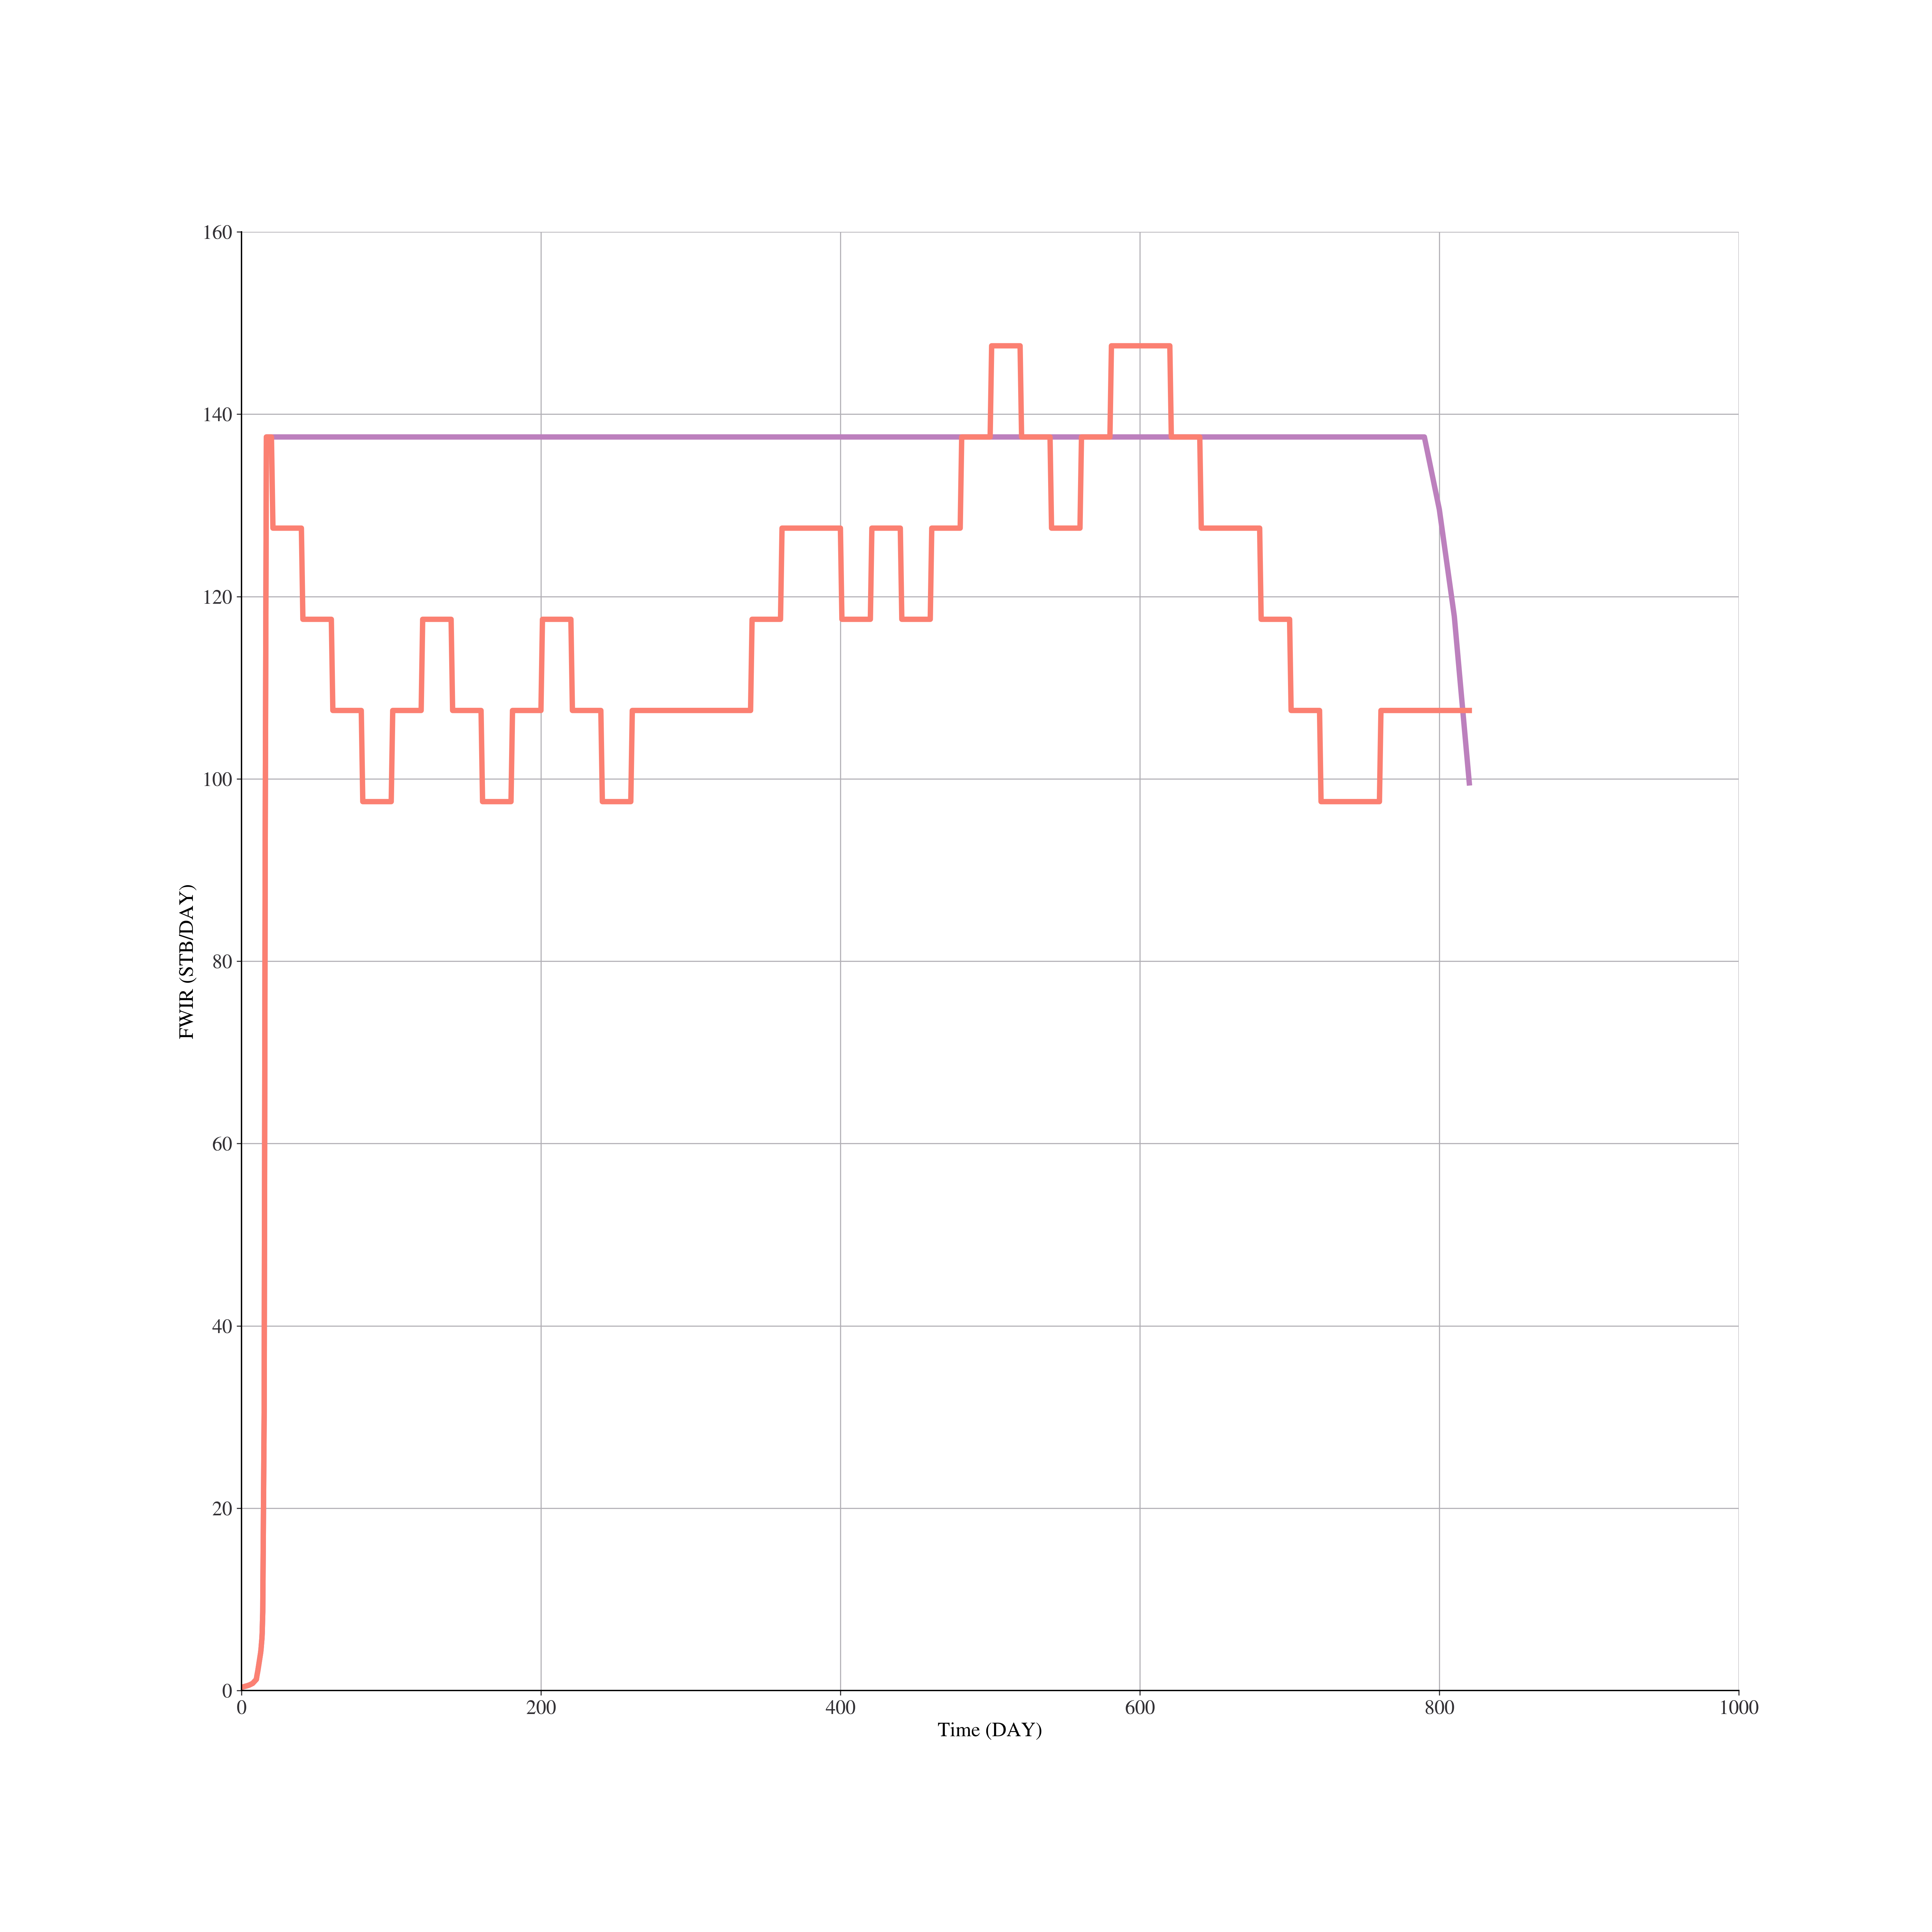
\includegraphics[width =\textwidth]{figures/prescriptive_analysis/FWIR (1).png}
    \caption{Field water injection total versus time}
    \label{fig:FWIT}
\end{figure}

The main aspect that explains the success of this policy is that it is able to minimize the cumulative heat loss to the surrounding rocks. Fig \ref{fig:FHLT} and \ref{fig:FHLR} show the rate of heat loss and cumulative loss to surrounding rocks. It is obvious that the policy defined by the (A2C) agent to change steam injection rate exhibits less heat loss to the surrounding rocks compared to the base case. This effect explains the success of this policy on water injection for optimizing oil recovery.  

\begin{figure}
    \centering
    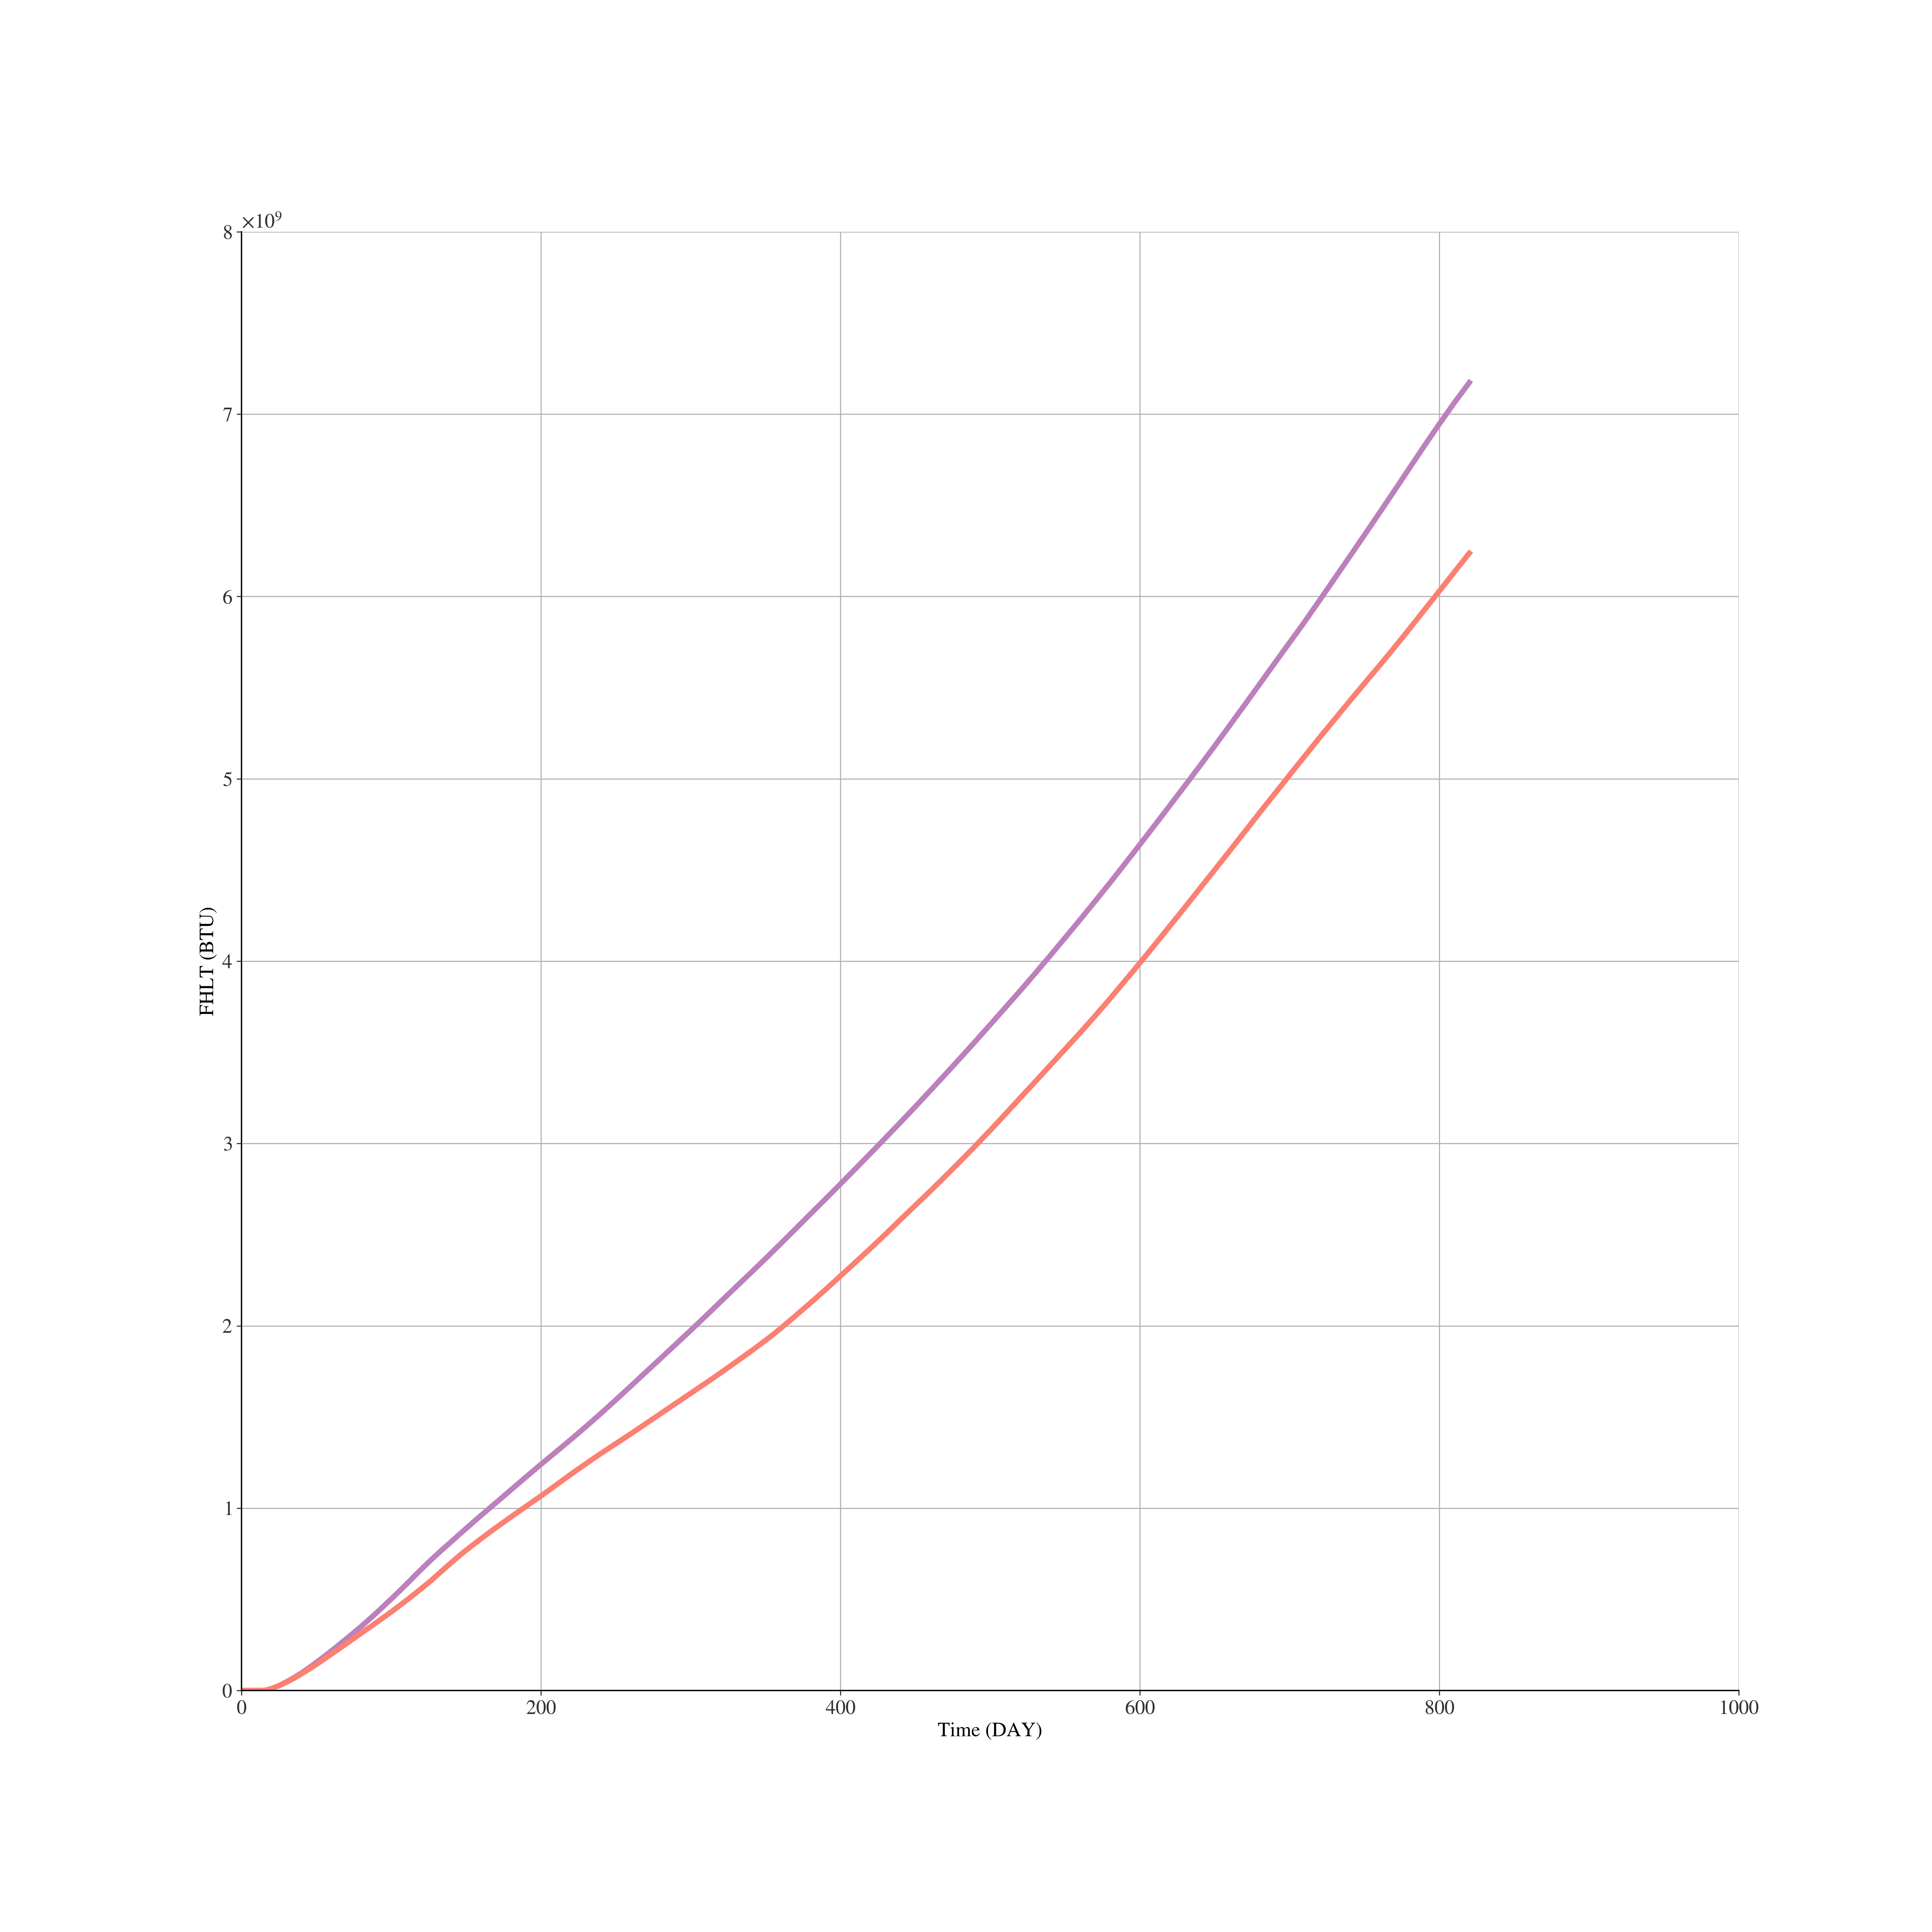
\includegraphics[width=\textwidth]{figures/prescriptive_analysis/FHLT (1).png}
    \caption{Field heat losses versus time}
    \label{fig:FHLT}
\end{figure}

\begin{figure}
    \centering
    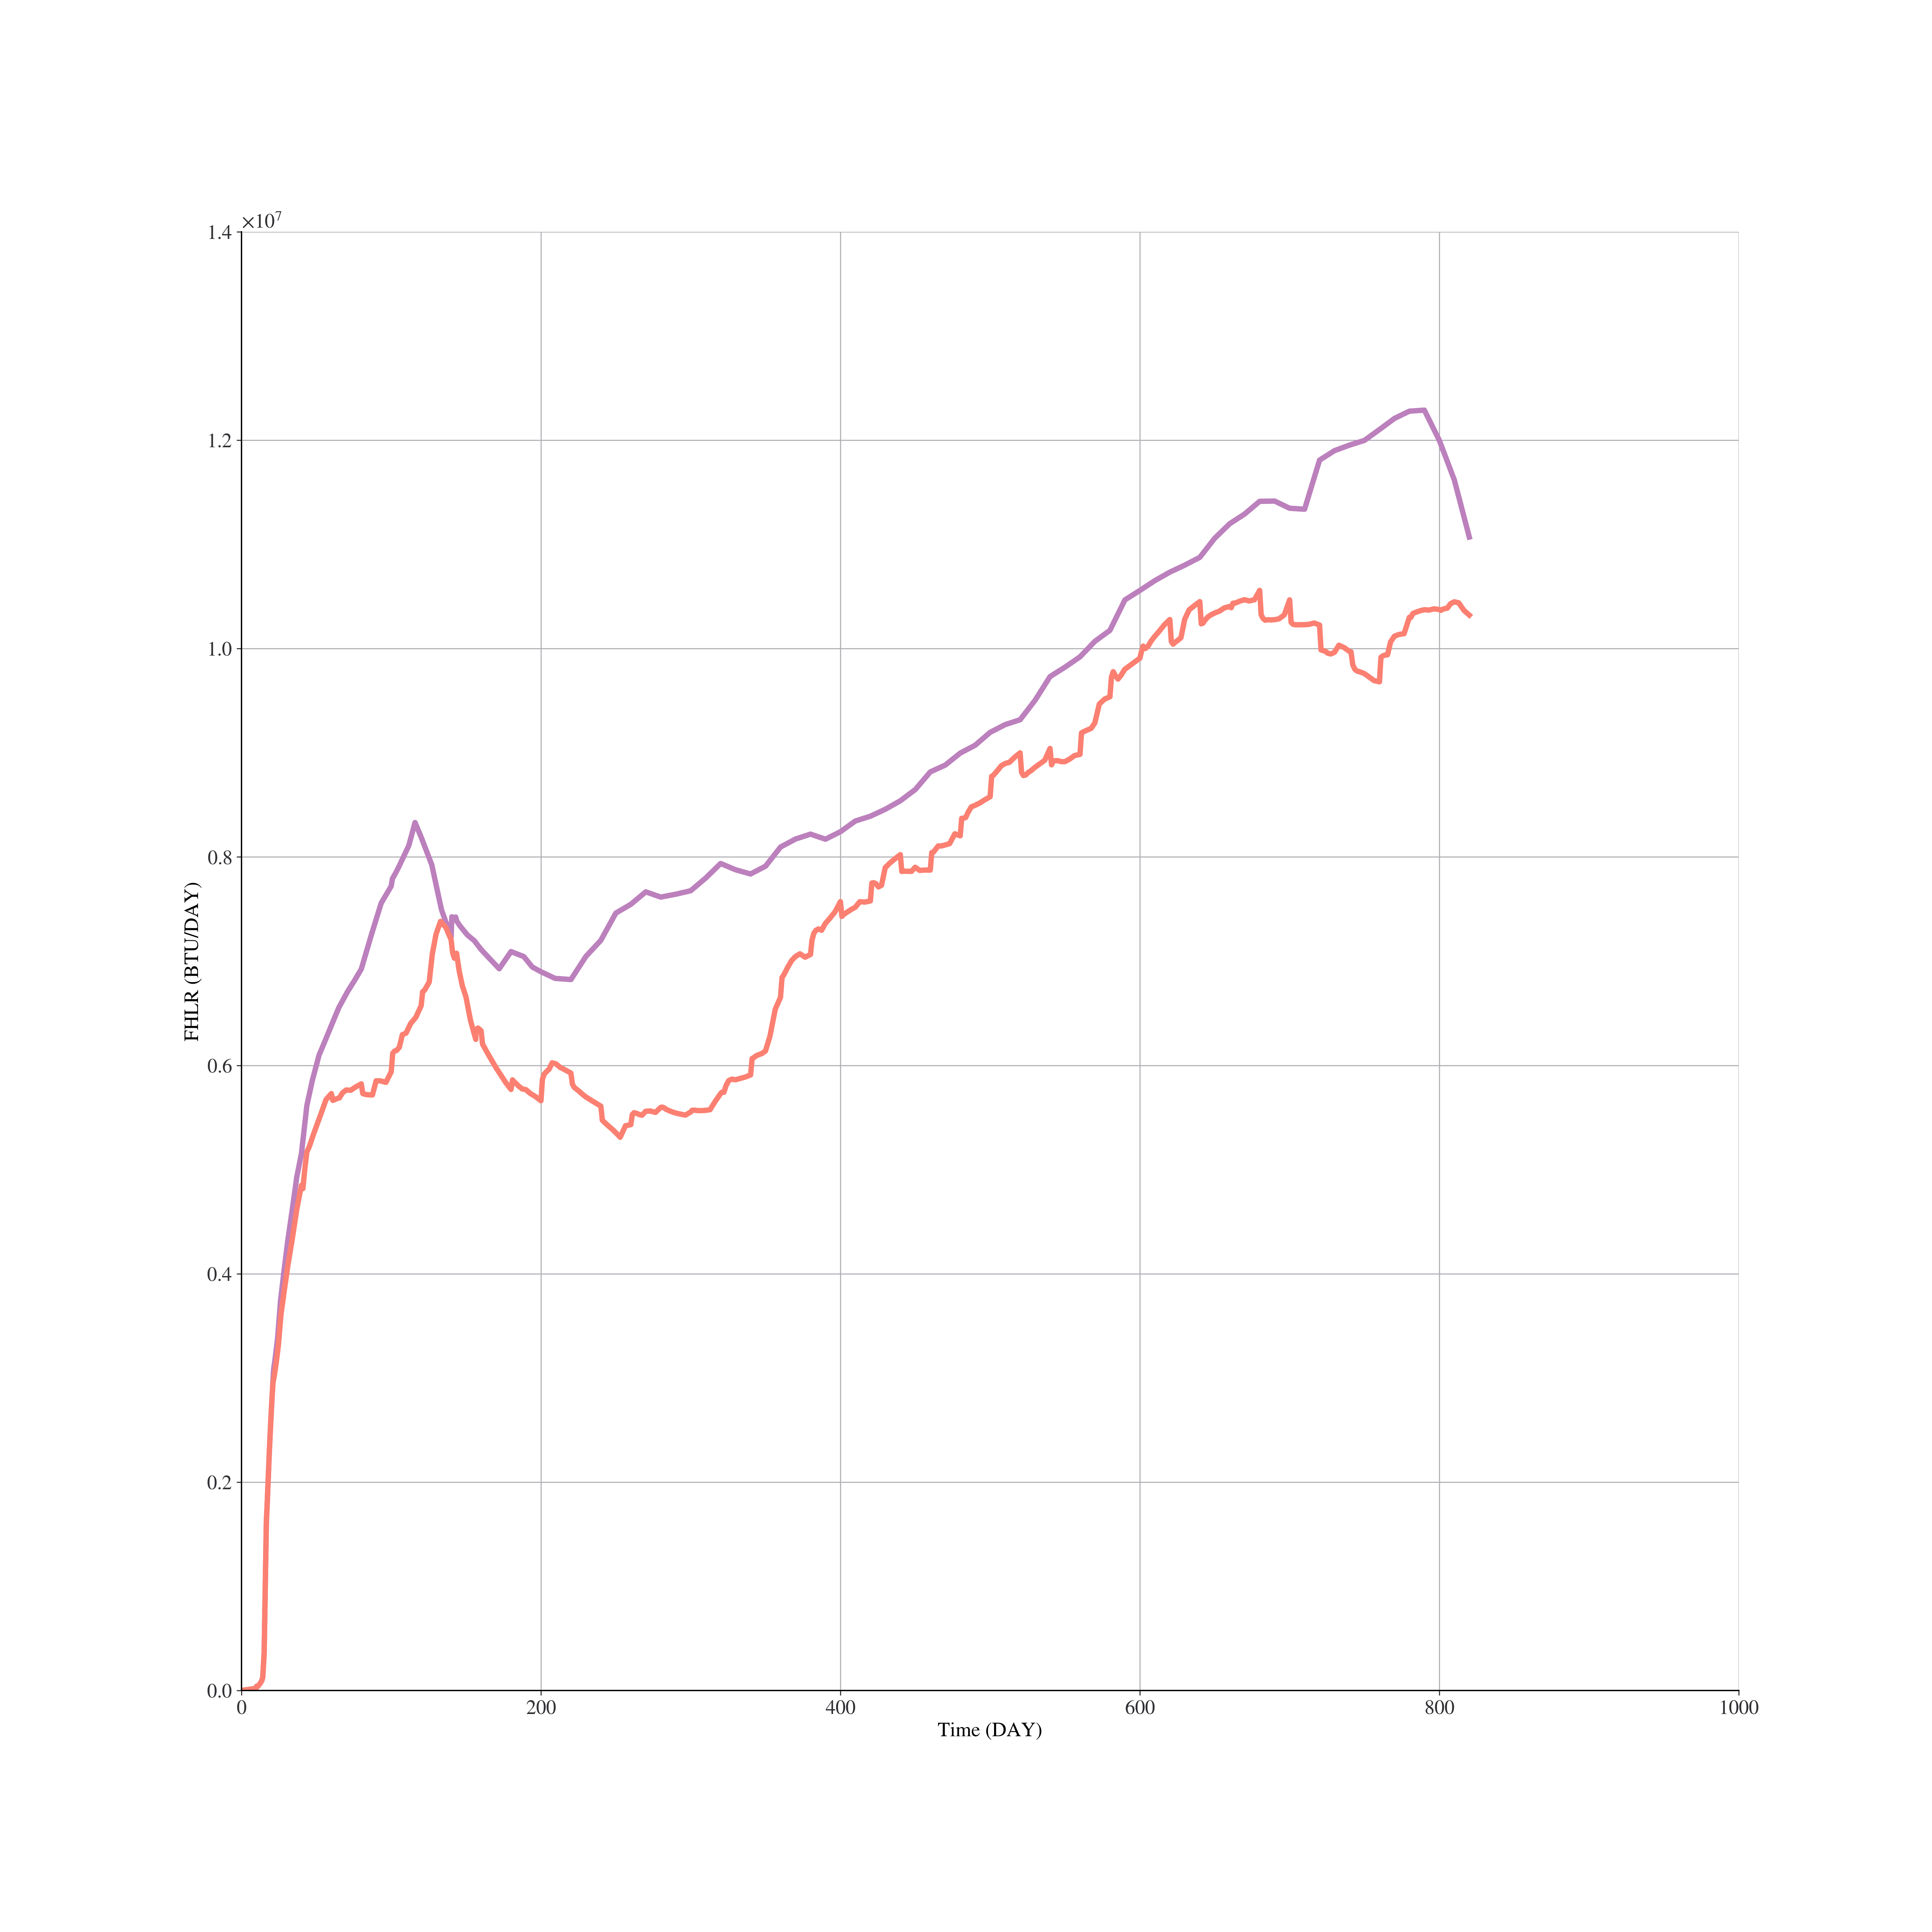
\includegraphics[width=\textwidth]{figures/prescriptive_analysis/FHLR (1).png}
    \caption{Field heat losses versus time}
    \label{fig:FHLR}
\end{figure}

Also it is important to study the effect of this injection policy on the produced oil and water. From Figures (11-12), it is shown that total water cut and the cumulative water production are less in the agent policy case than the base case. This may be an effect of slightly smaller injection rates at the first region of the production horizon that leads to the steam chamber to grew vertically. 

\begin{figure}
    \centering
    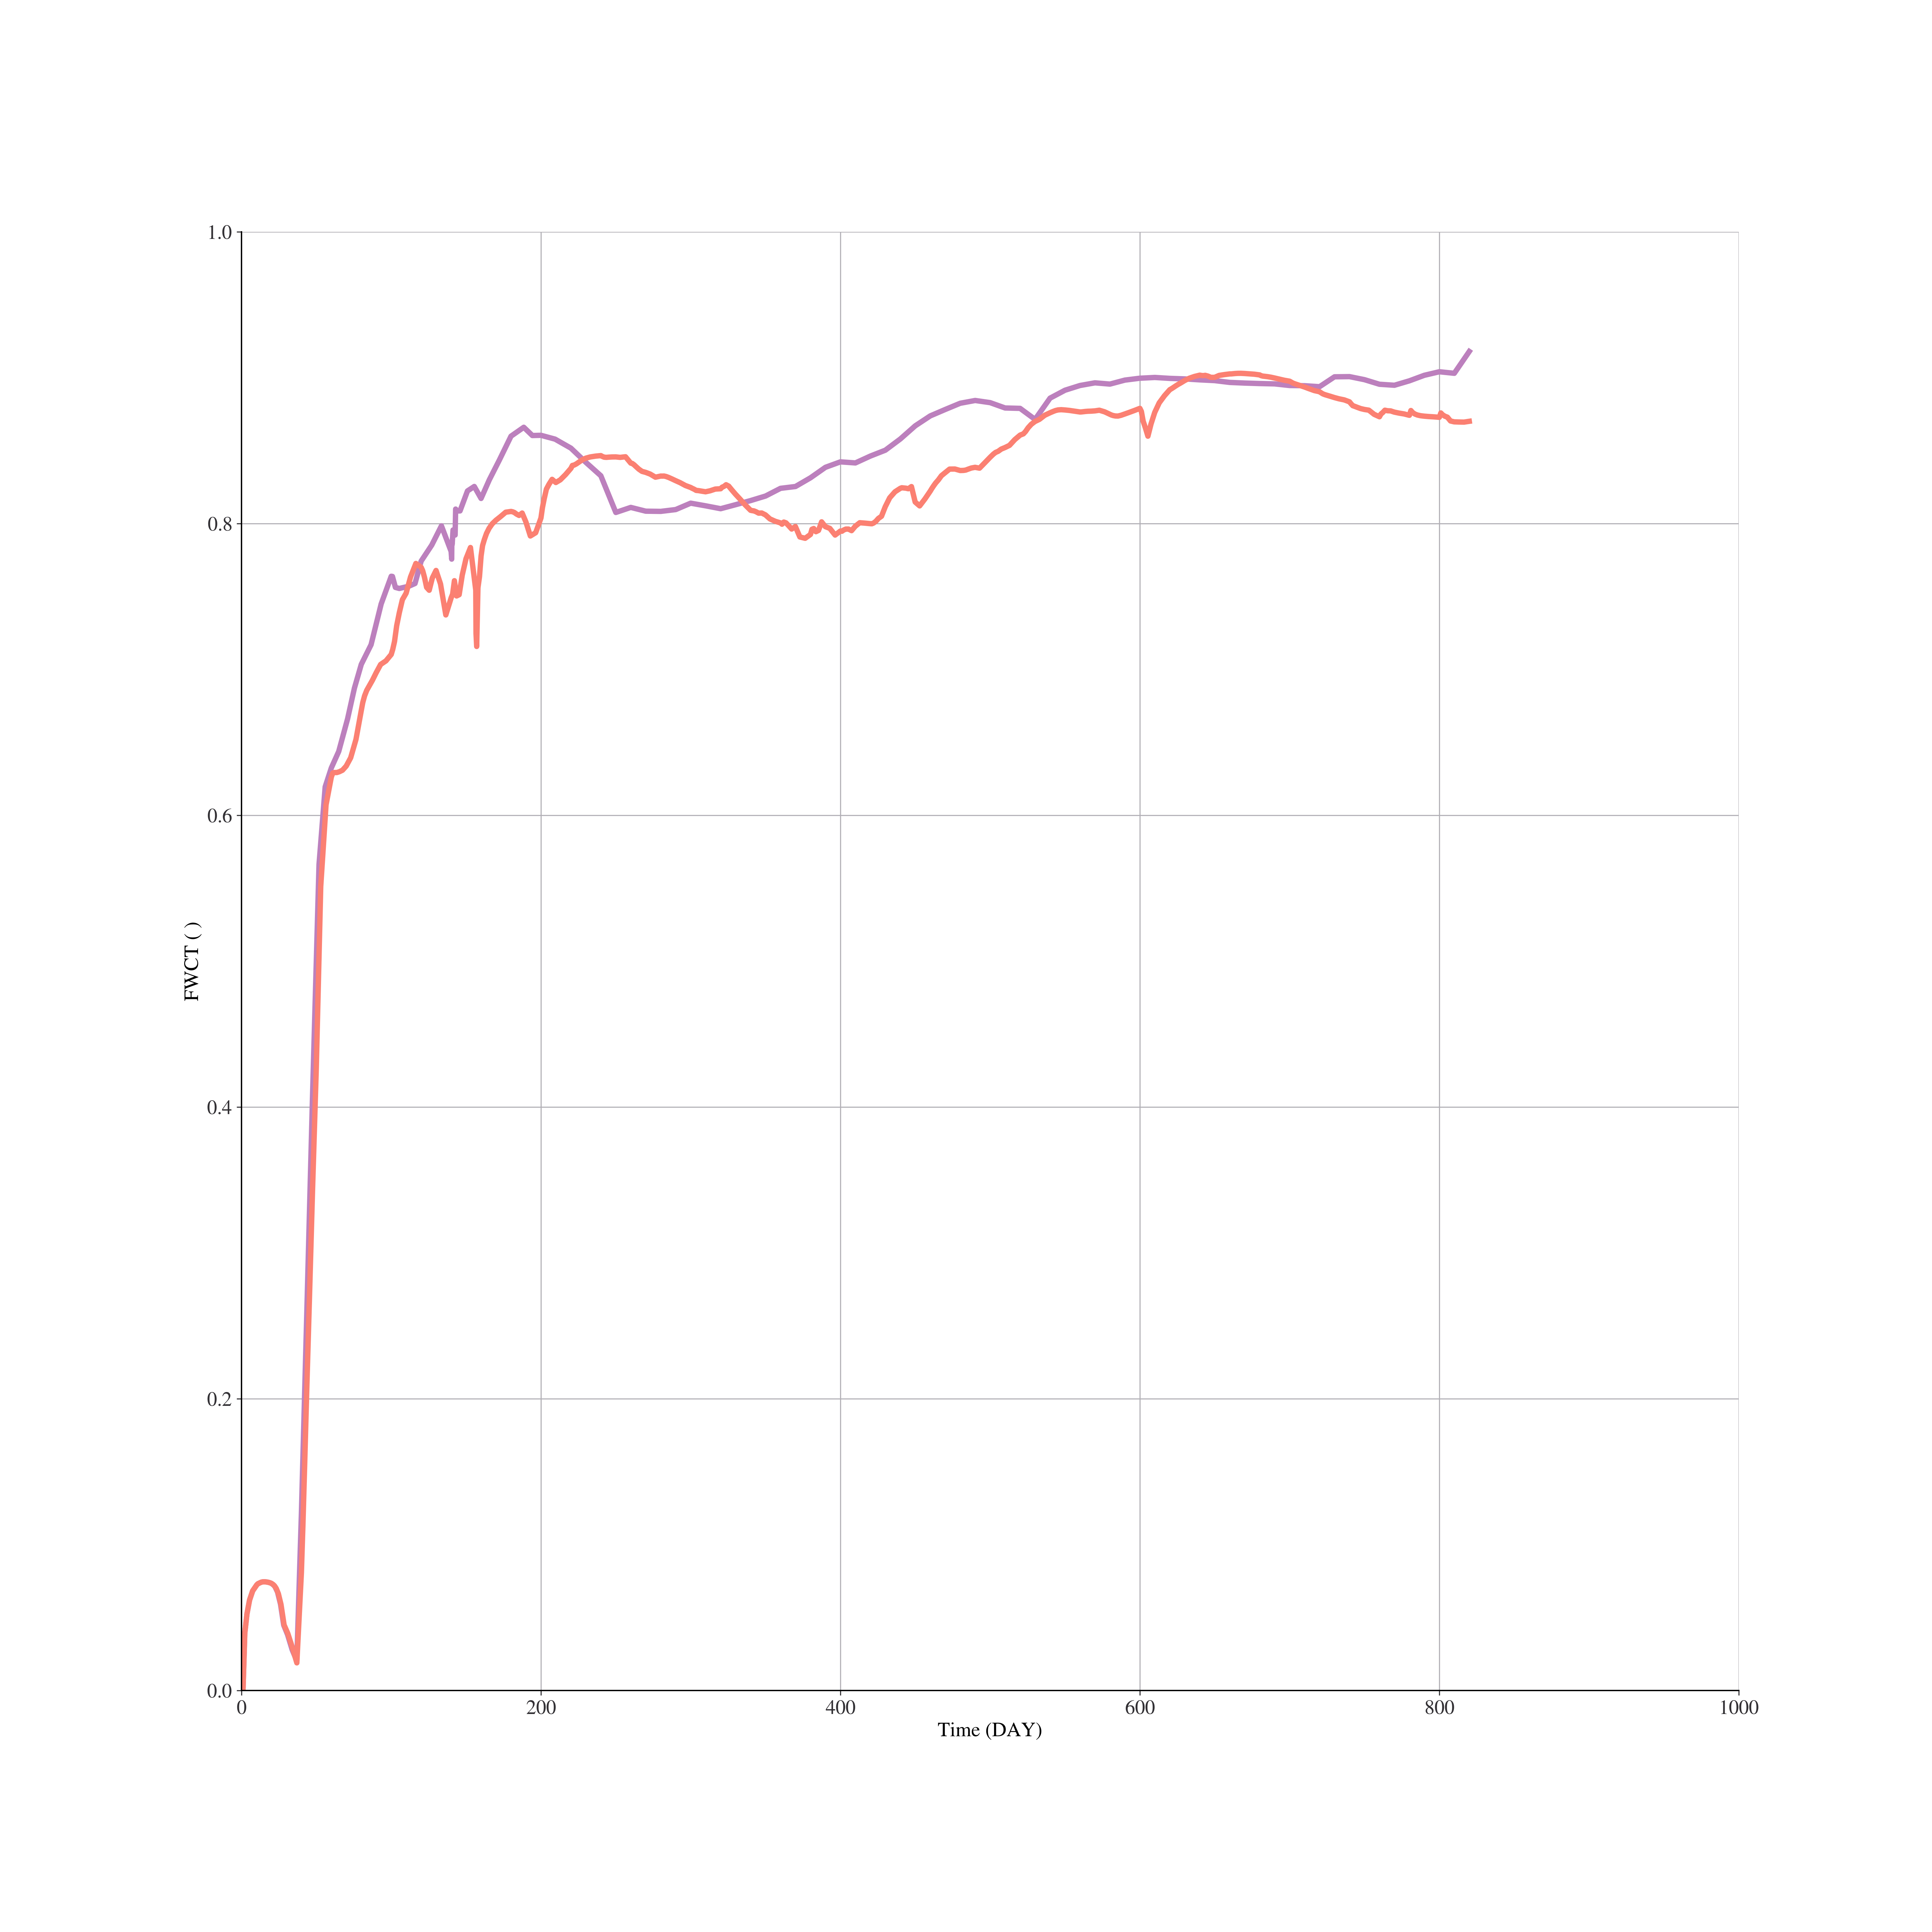
\includegraphics[width=\textwidth]{figures/prescriptive_analysis/FWCT (1).png}
    \caption{Field water cut versus time}
    \label{fig:FWCT}
\end{figure}

\begin{figure}
    \centering
    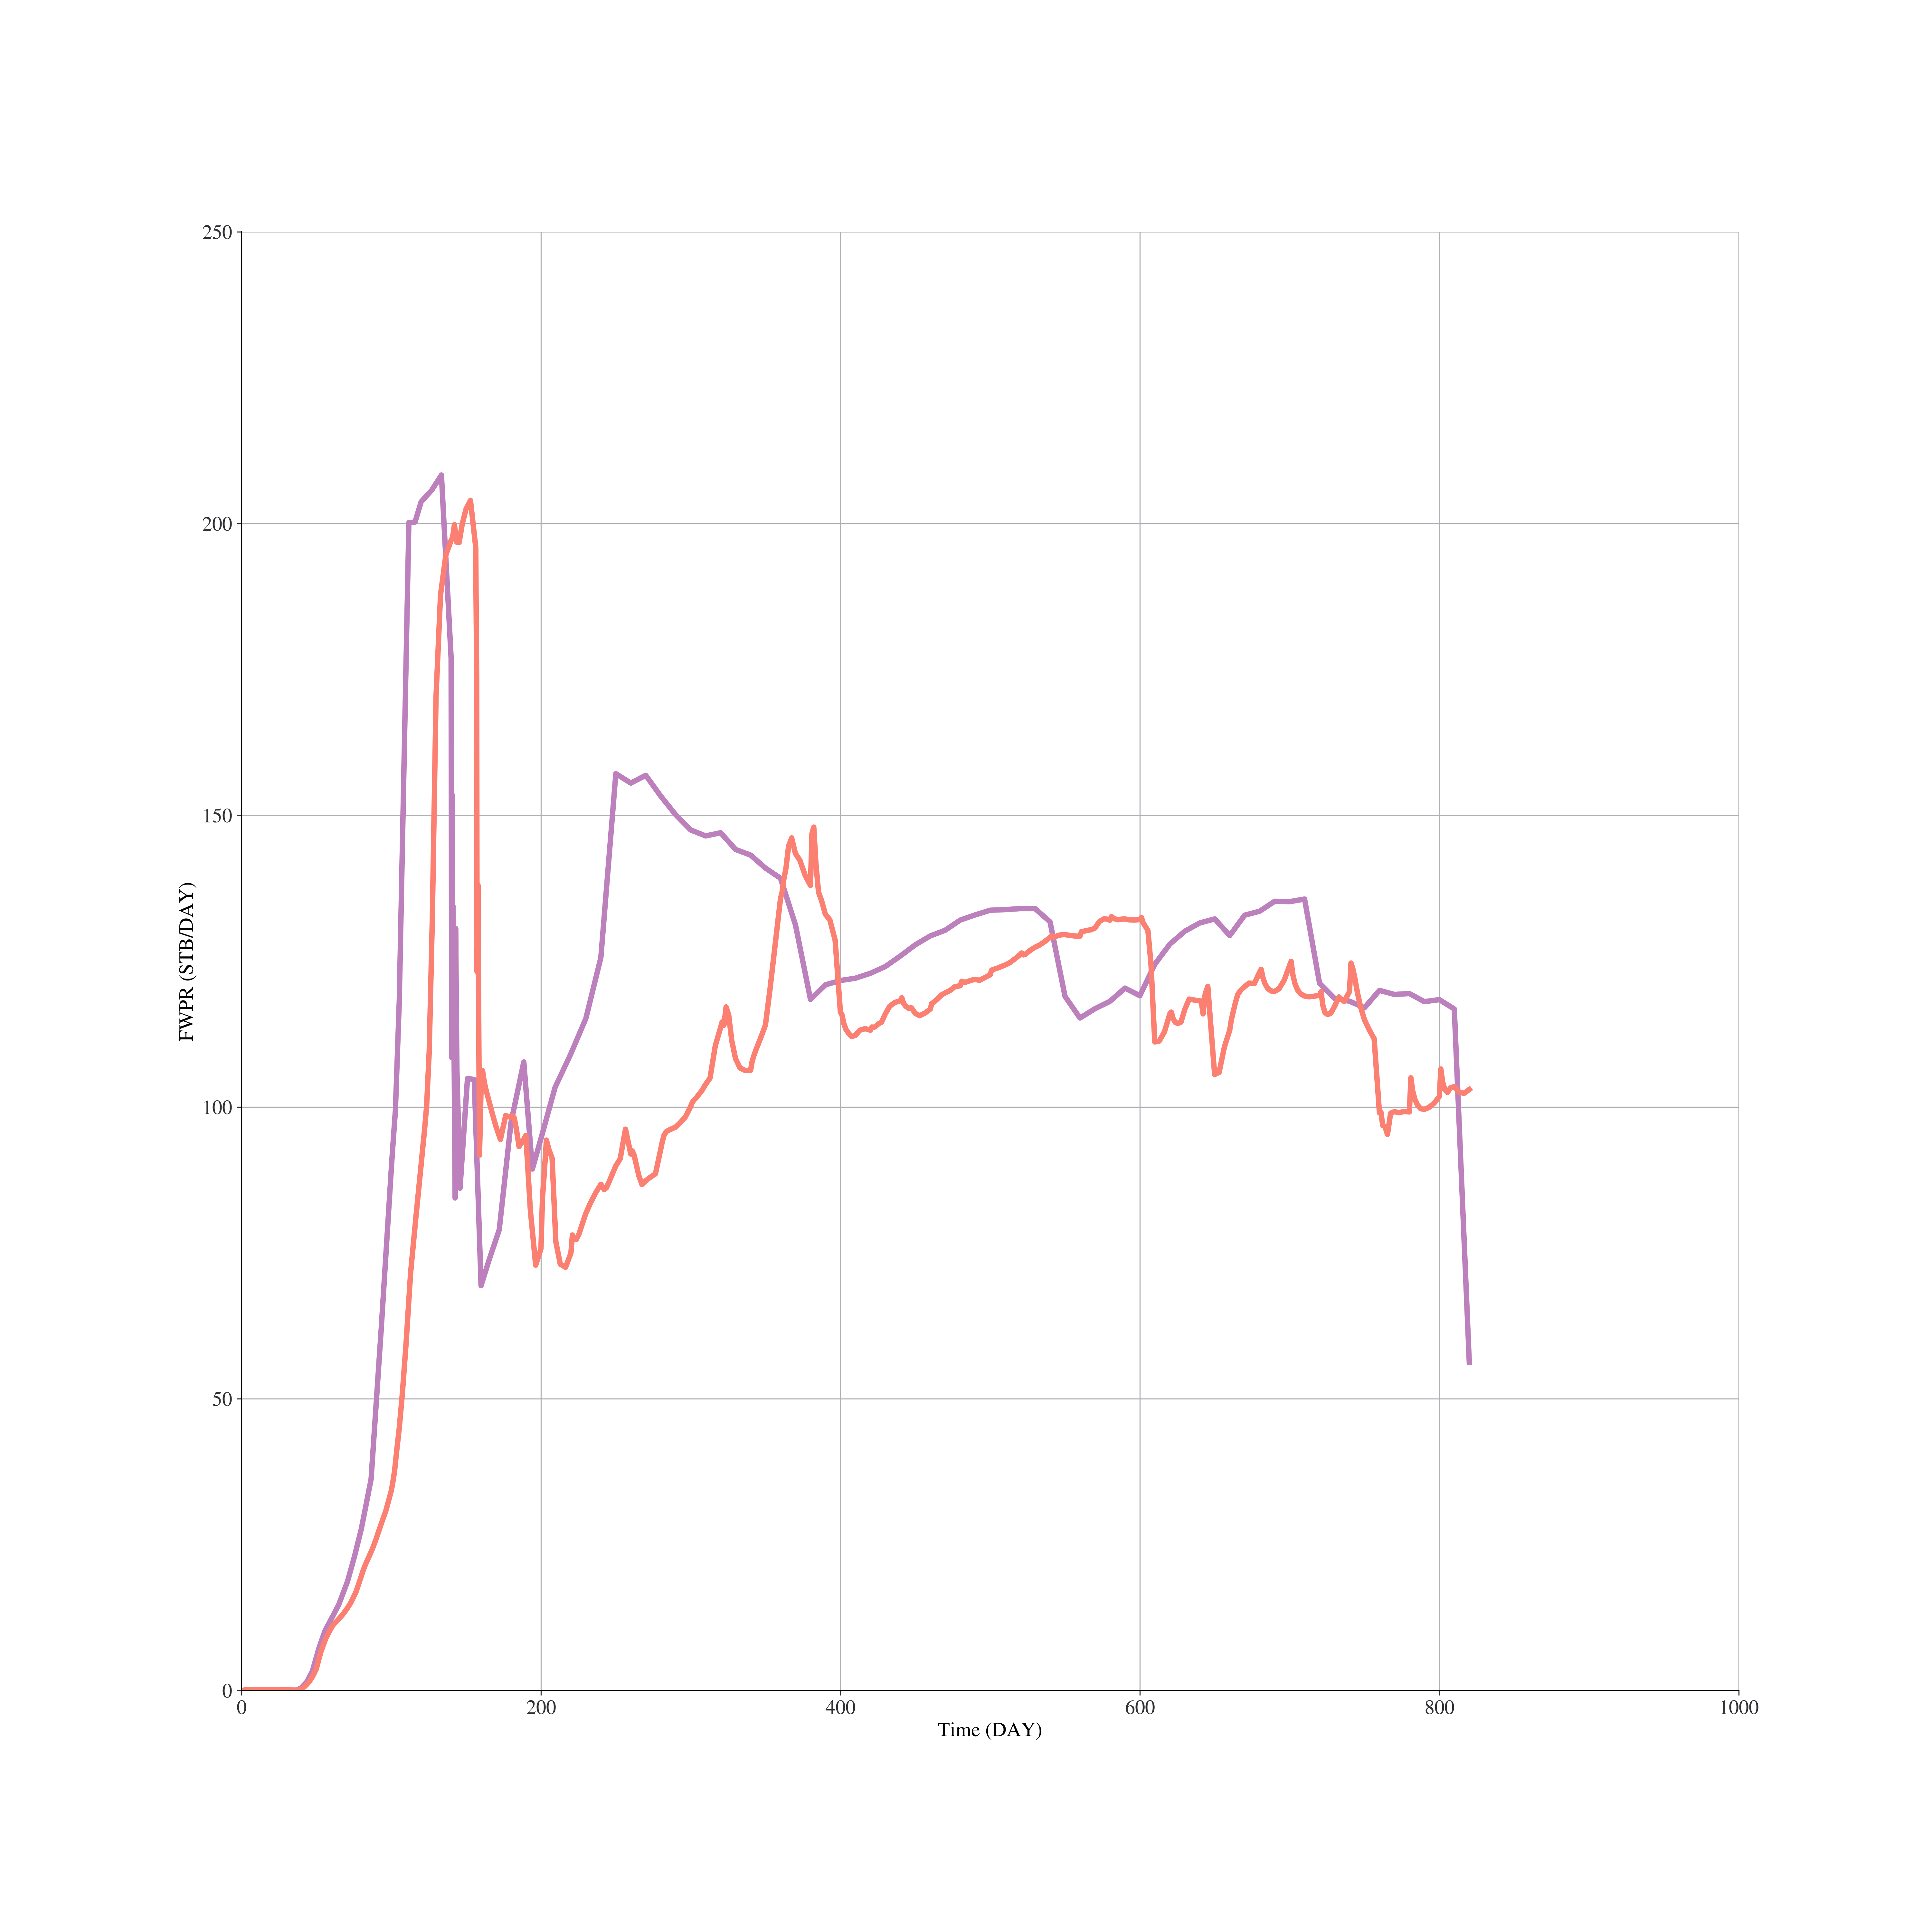
\includegraphics[width=\textwidth]{figures/prescriptive_analysis/FWPR (1).png}
    \caption{ Cumulative water production versus time}
    \label{fig:FWPR}
\end{figure}

Figure 12-13 shows the oil rate and cumulative oil production versus time. It is shown that the agent policy shifted the profile of oil production rate. The second peak shifted from day 260 to day 400. In the A2C policy this leads to reduce the sharp decrease happening afterwards and also leads to delay the steam breakthrough in the near and far wells. Fig 14 and 15 show the total steam production from the near and far wells in both A2C and base cases. While the near well starts to produce steam after 160 days in the A2C case while in the base case it starts to produce steam after 140 days. The same happens for the far well with approximately 80 days difference.

\begin{figure}
    \centering
    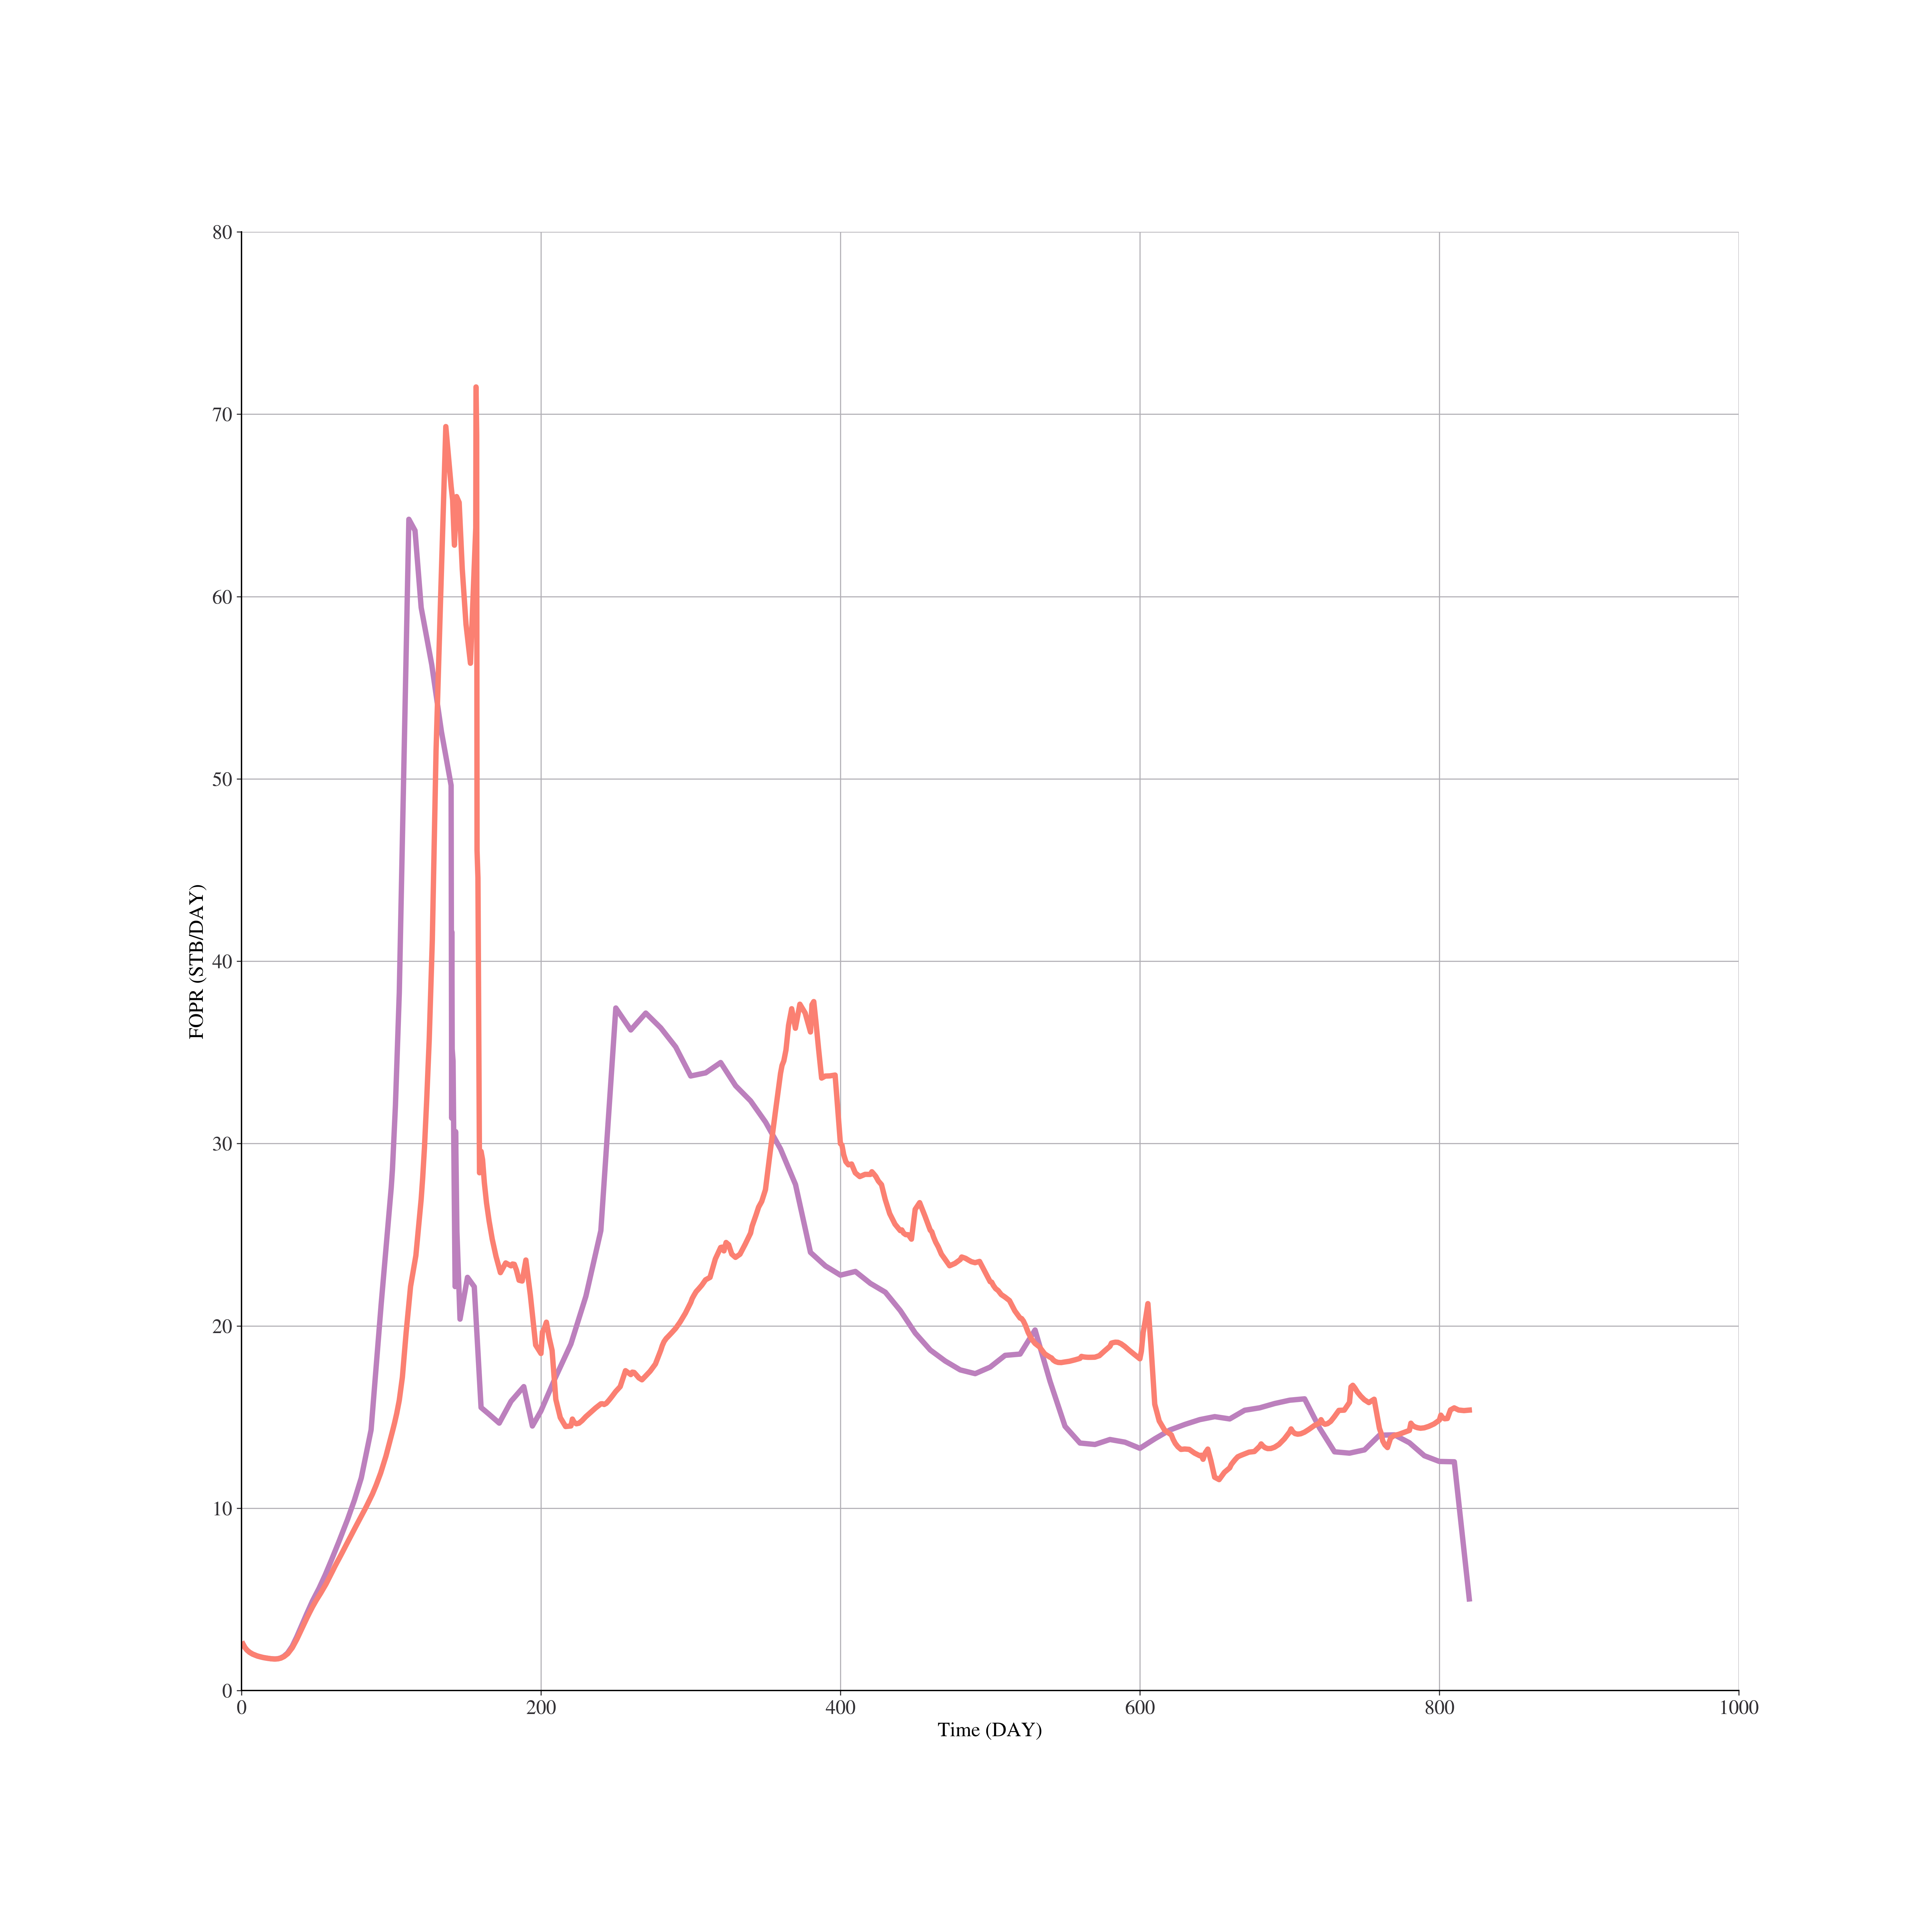
\includegraphics[width=\textwidth]{figures/prescriptive_analysis/FOPR (1).png}
    \caption{ Field oil production rate versus time}
    \label{fig:FOPR}
\end{figure}

\begin{figure}
    \centering
    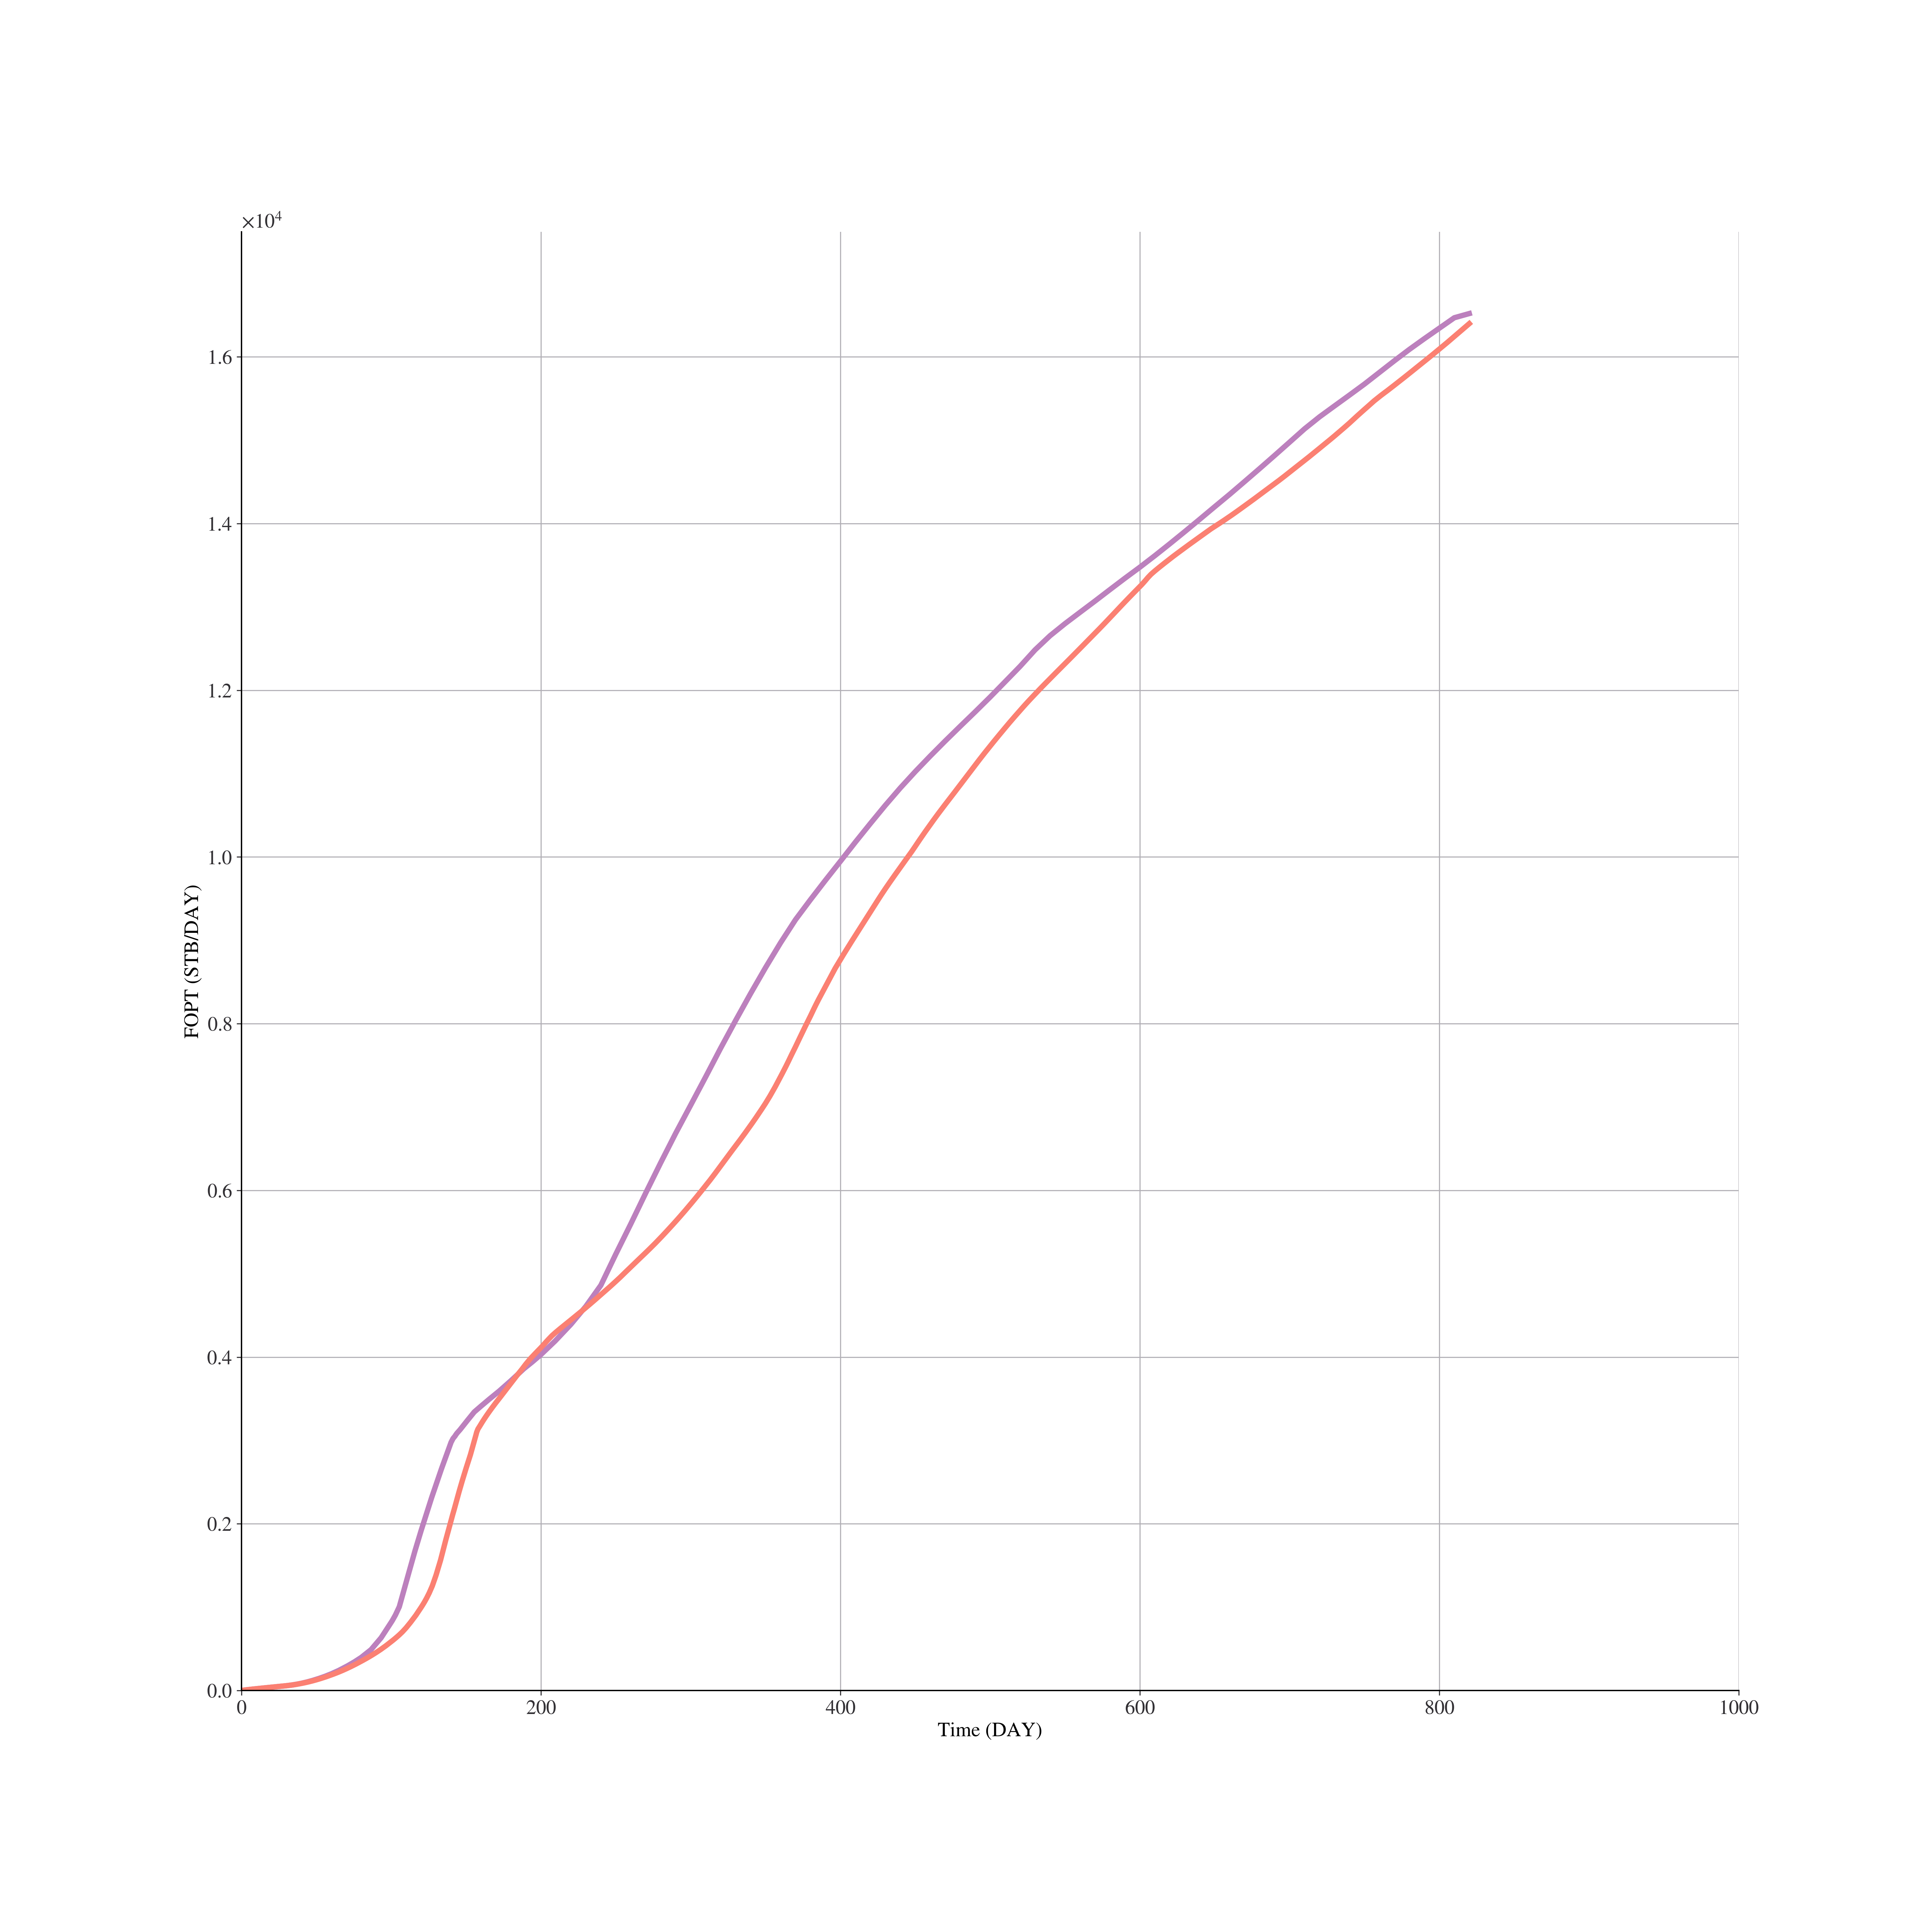
\includegraphics[width=\textwidth]{figures/prescriptive_analysis/FOPT (1).png}
    \caption{ Cumulative water production versus time}
    \label{fig:FOPT}
\end{figure}

\begin{figure}
    \centering
    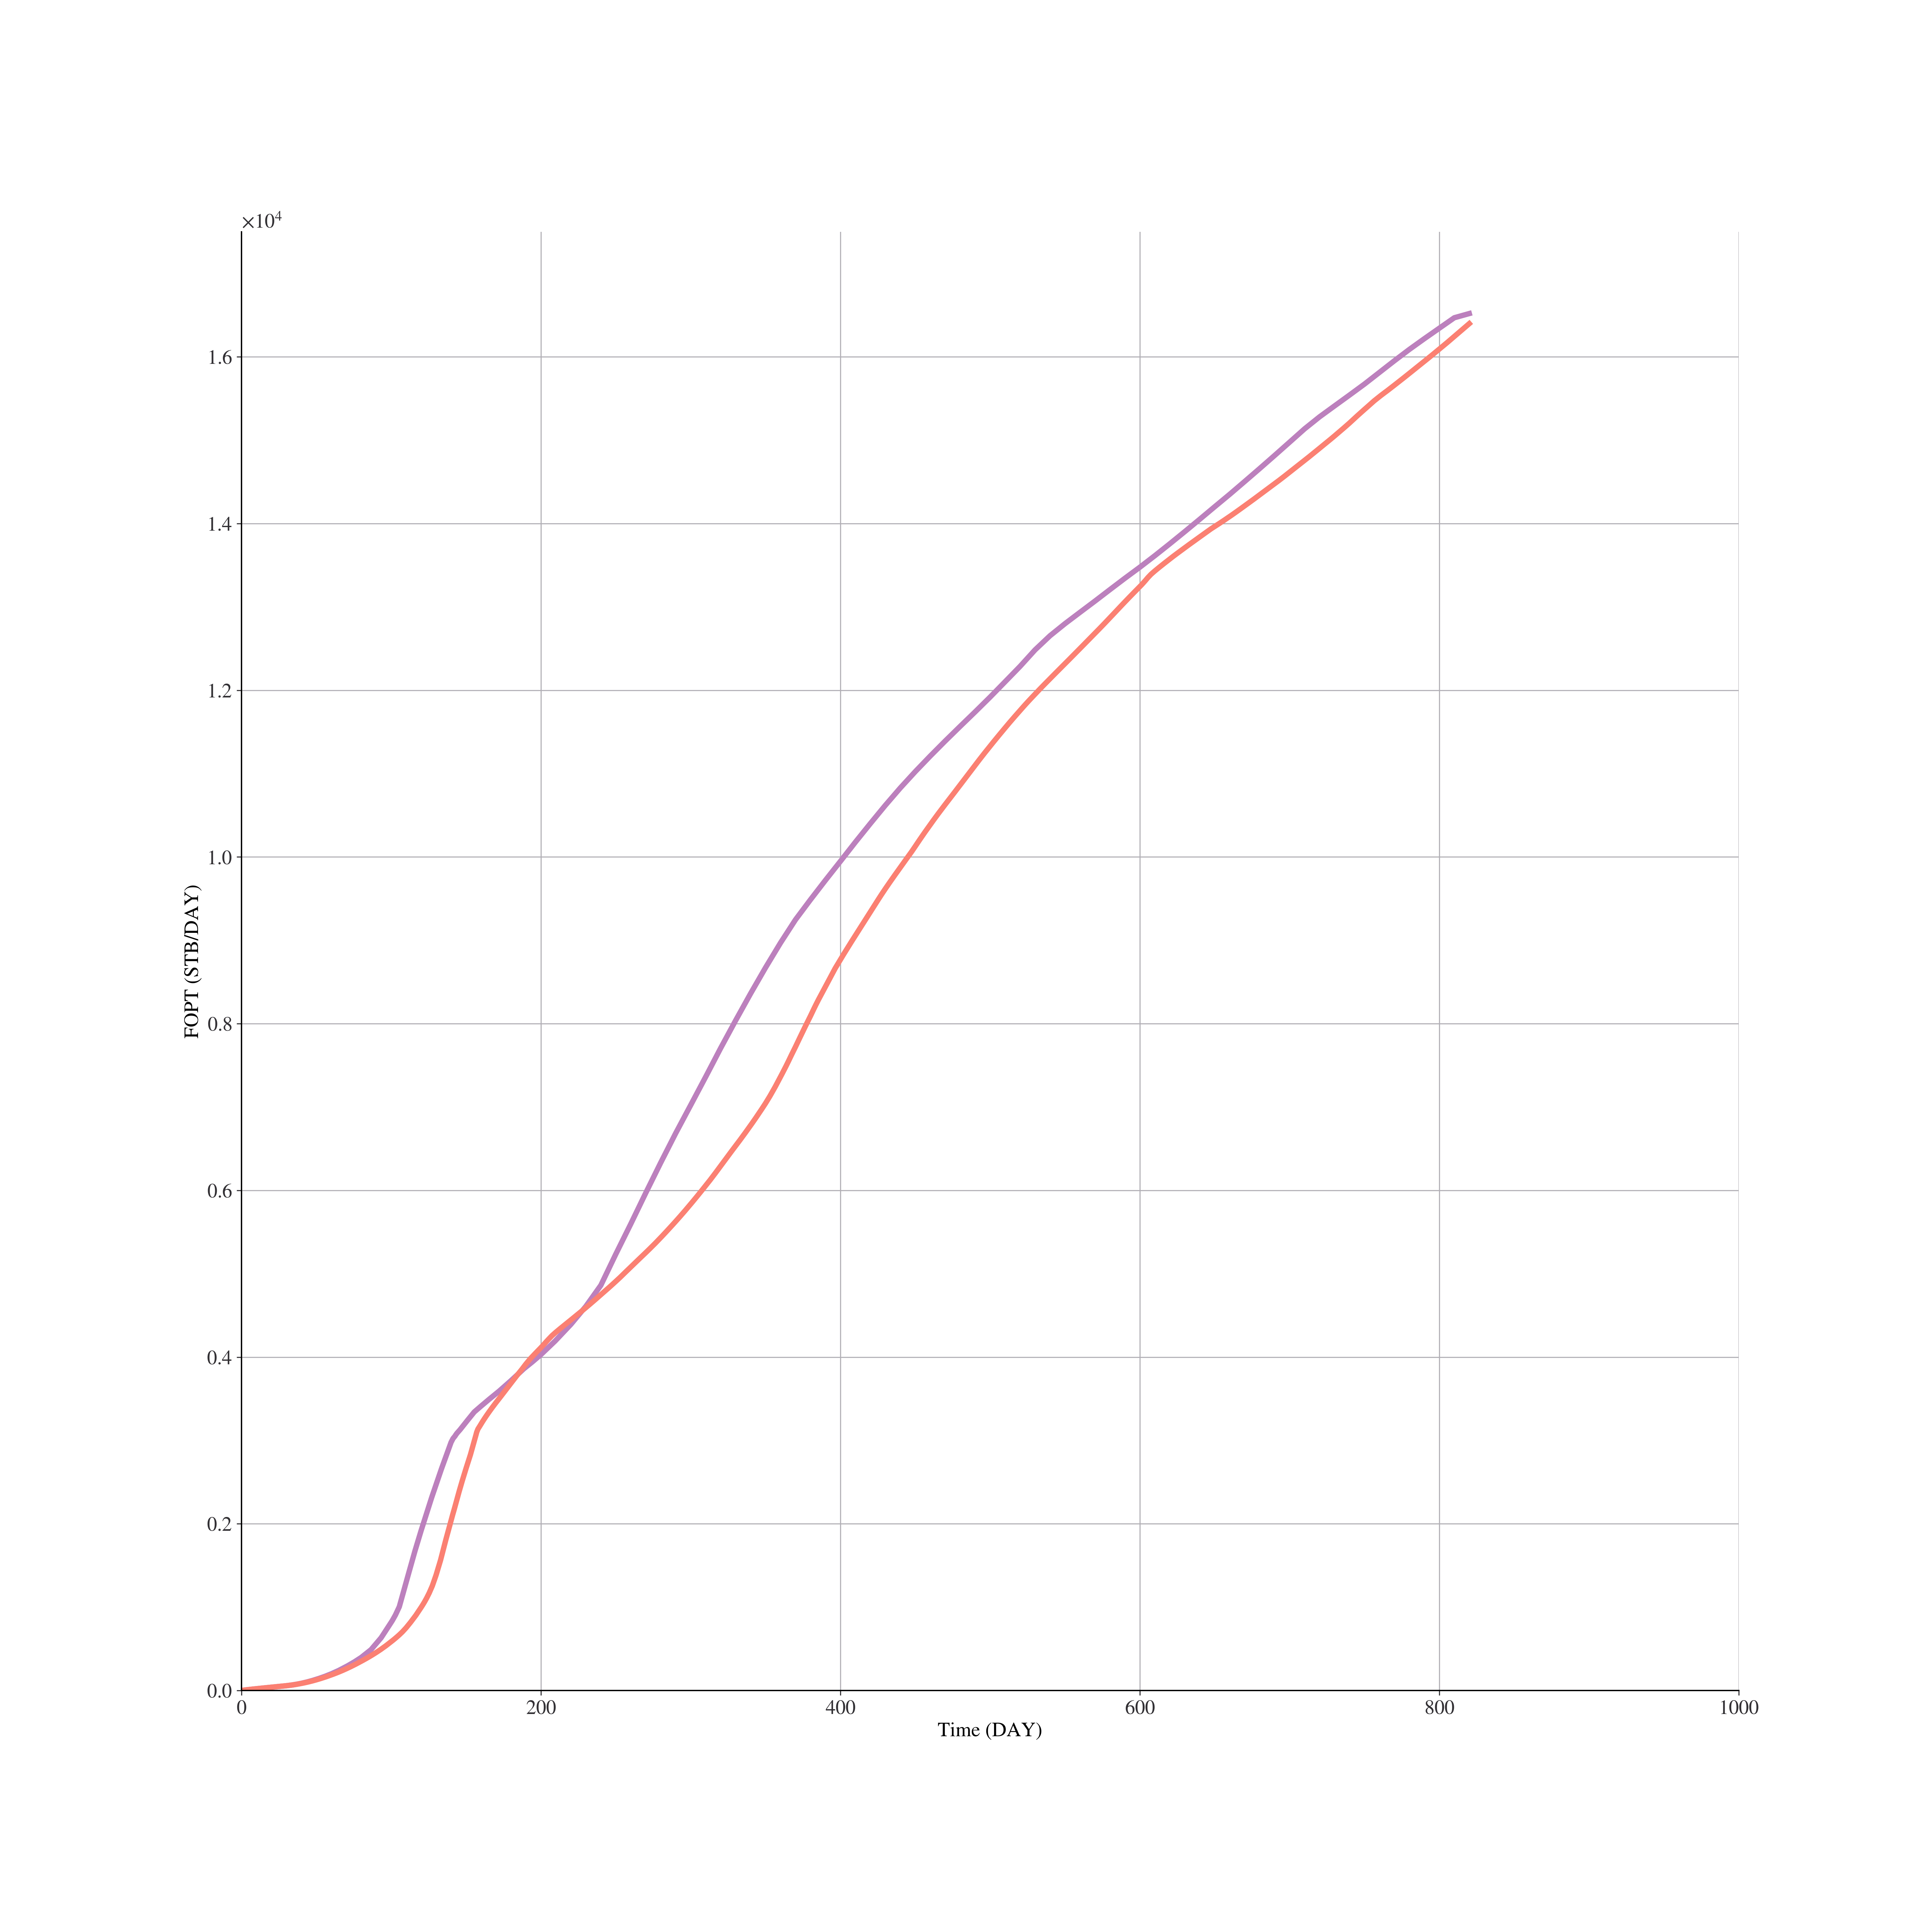
\includegraphics[width=\textwidth]{figures/prescriptive_analysis/FOPT (1).png}
    \caption{ Cumulative Steam Production in the near production well}
    \label{fig:FW}
\end{figure}

 \begin{figure}
    \centering
    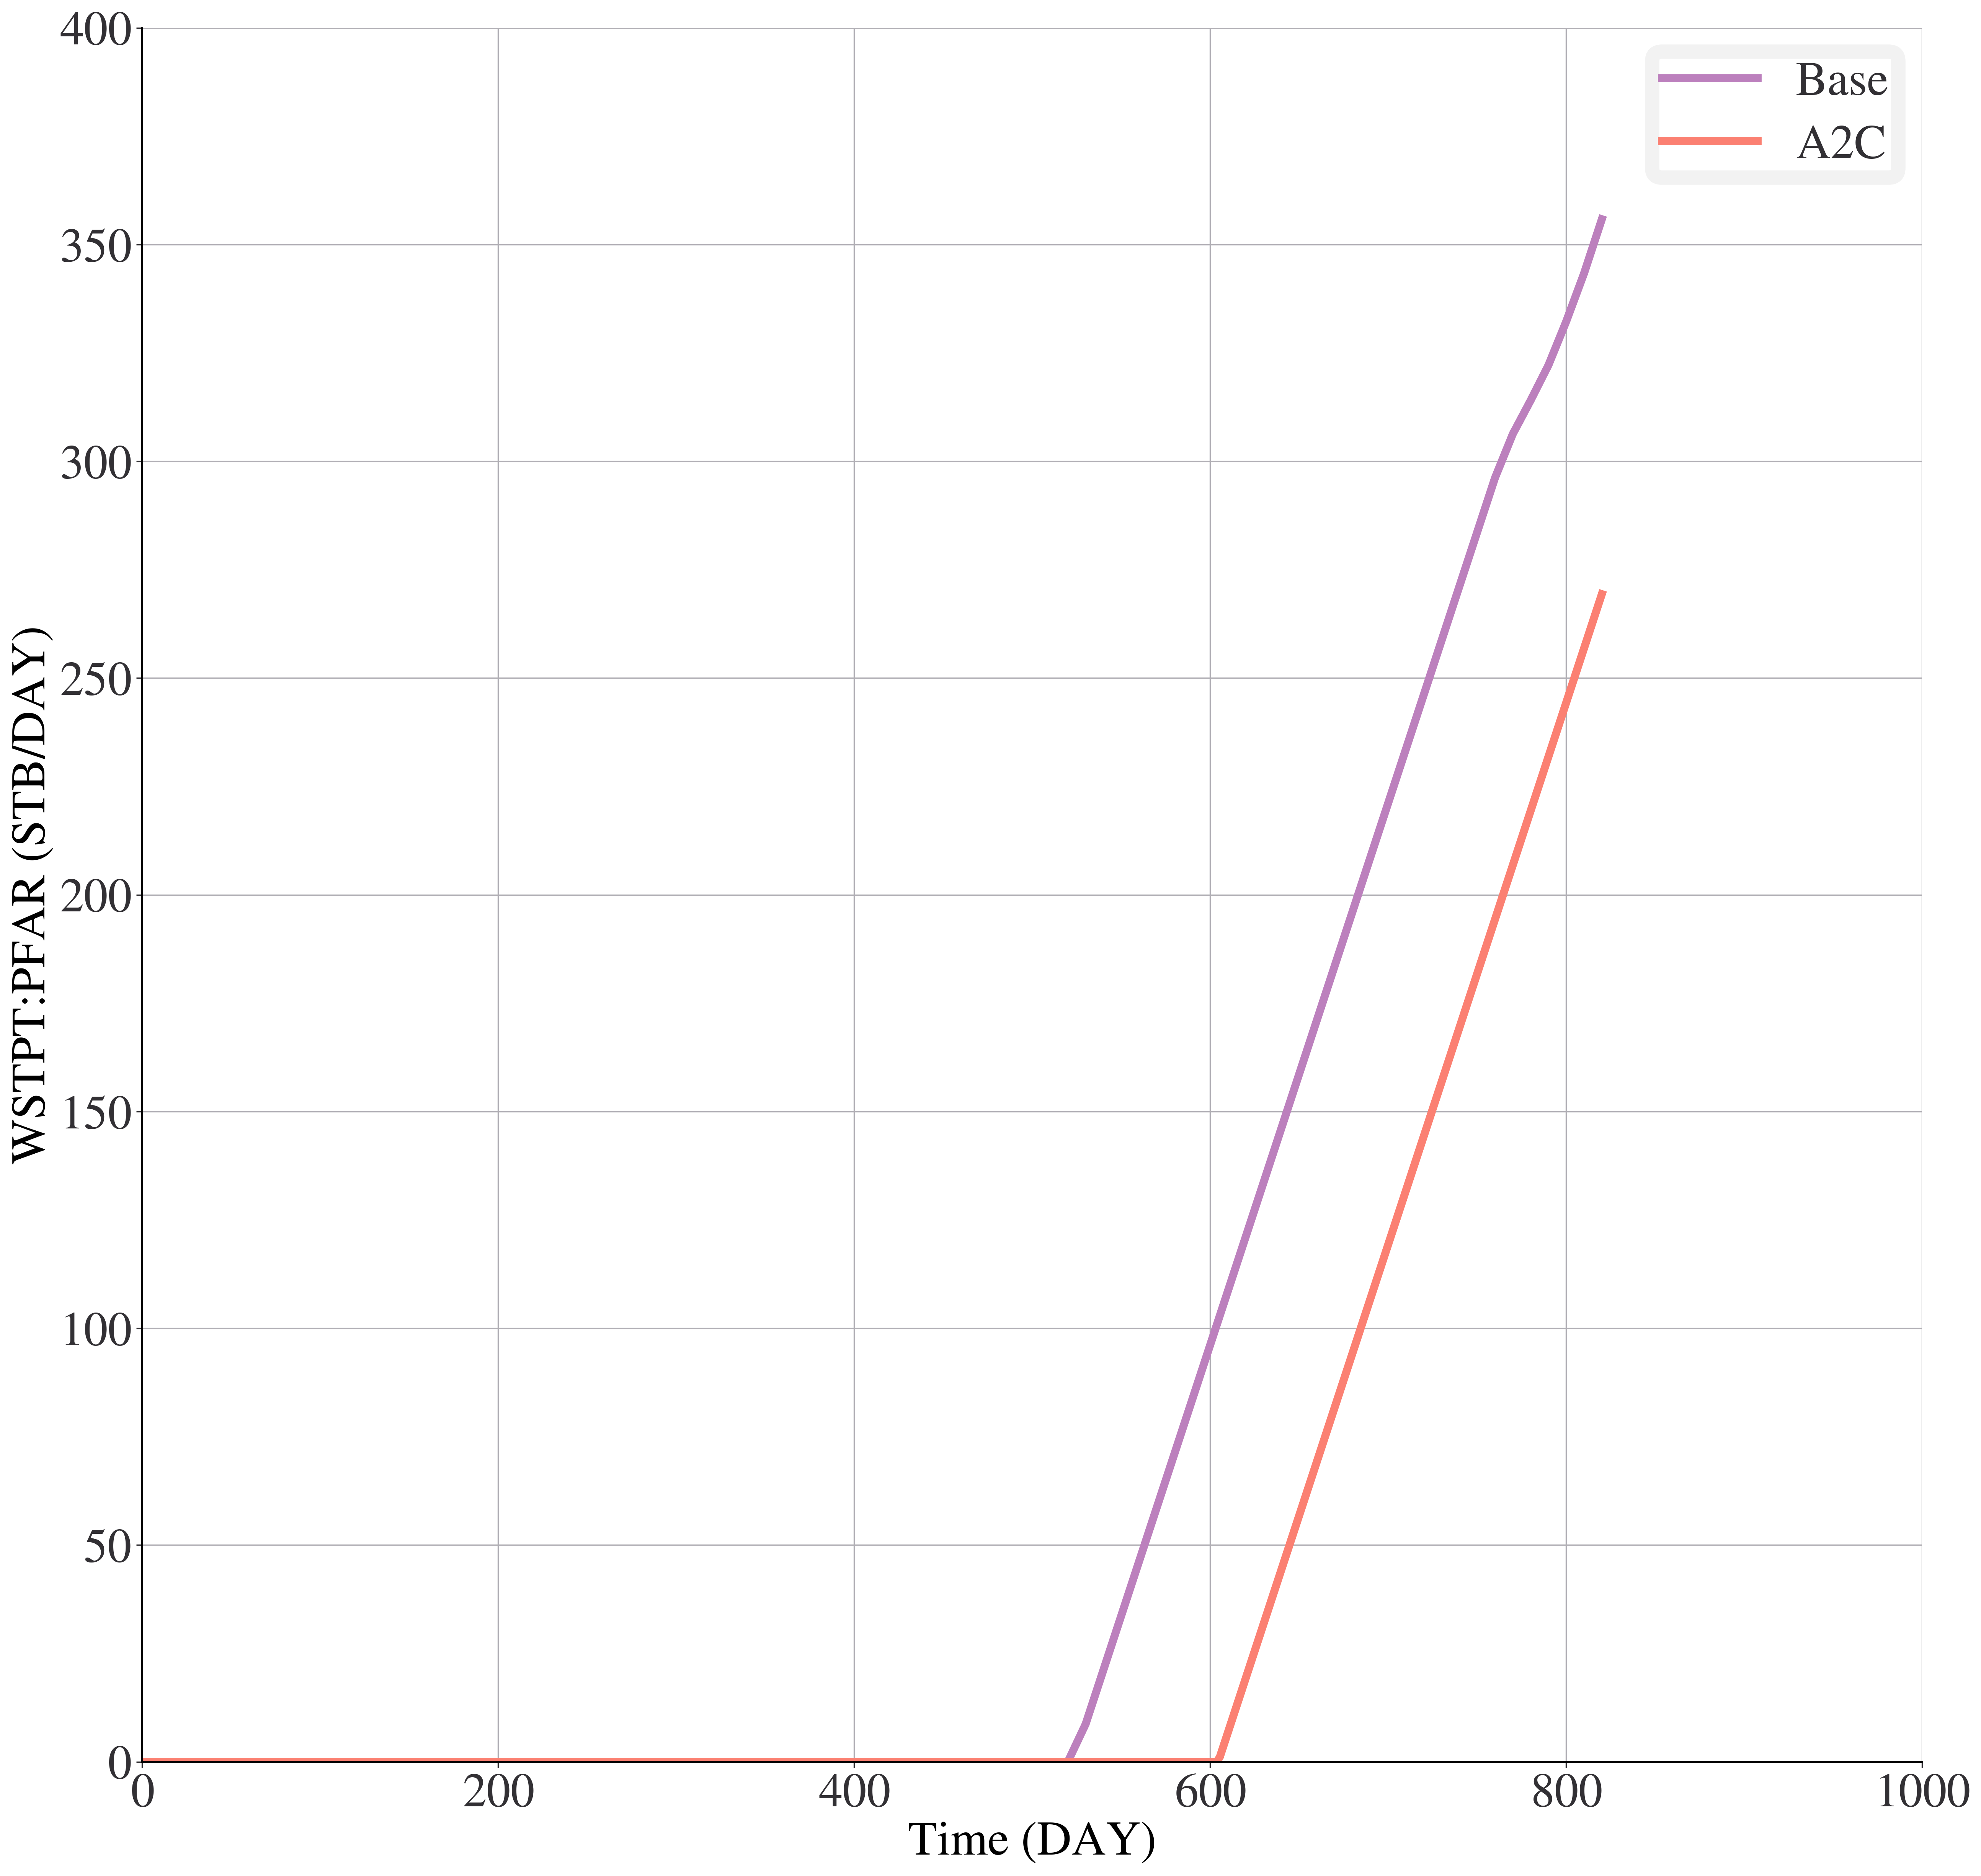
\includegraphics[width=\textwidth]{figures/prescriptive_analysis/steam3.png}
    \caption{Cumulative Steam production in the far production well}
    \label{fig:FWCT}
\end{figure}

\section{Discussion}
From the results of this study, it can be observed that the constructed ANN model is more accurate than SVM model. That is why the constructed ANN model was utilized to measure the precession and recall with respect to rod pump conditions rather than SVM model. This precedence of the ANN model over the SVM model in the rod pump conditions prediction might be due the nature of the data that were utilized, and also the way the constructed models were designed. Otherwise, in some cases or some other fields of study, SVM model may produce better accuracy than ANN model. 

The constructed ANN models have to be developed and optimized with several scenarios of learning rate, momentum, number of nodes in the hidden layer and activation functions, since in each case during this study different scenarios achieved the different accuracy of prediction. Therefore, the program has to be designed and optimized in such a way that it can produce the best prediction by combining the most optimum parameters.

After the best network structure was selected, the proposed model was evaluated. Evaluation was made by getting precision and recall values for testing dataset. 958 dynamometer cards for various pumping conditions were considered in the testing dataset. These cards were not used in either training or validation of the model.

Beyond the accuracy value, the weighted average of Precision and Recall was calculated. This value is called F1 Score. In this research, F1 Score is 89.5%. Therefore, this score takes both false positives and false negatives into account. F1 Score is usually more useful than accuracy, especially if you have an uneven class distribution. 

From the field applications, the rod pump systems with only one problem can be detected easily with high degree of confidence. However, complex systems with multiple downhole rod pump problems are recognized with lower confidence level.

It should be highlighted that the use of machine learning in rod pump diagnosis has the advantage of less human interaction. The developed model can interpret large number of dynamometer cards automatically and it lends itself to digital oil field applications.